% Generated by Sphinx.
\def\sphinxdocclass{article}
\documentclass[letterpaper,10pt,english]{sphinxhowto}
\usepackage[utf8]{inputenc}
\DeclareUnicodeCharacter{00A0}{\nobreakspace}
\usepackage[T1]{fontenc}
\usepackage{babel}
\usepackage{times}
\usepackage[Bjarne]{fncychap}
\usepackage{longtable}
\usepackage{sphinx}
\usepackage{multirow}


\title{COCOMA Documentation}
\date{June 06, 2013}
\release{1}
\author{Carmelo Ragusa, Philip Robinson, Sergej Svorobej}
\newcommand{\sphinxlogo}{}
\renewcommand{\releasename}{Release}
\makeindex

\makeatletter
\def\PYG@reset{\let\PYG@it=\relax \let\PYG@bf=\relax%
    \let\PYG@ul=\relax \let\PYG@tc=\relax%
    \let\PYG@bc=\relax \let\PYG@ff=\relax}
\def\PYG@tok#1{\csname PYG@tok@#1\endcsname}
\def\PYG@toks#1+{\ifx\relax#1\empty\else%
    \PYG@tok{#1}\expandafter\PYG@toks\fi}
\def\PYG@do#1{\PYG@bc{\PYG@tc{\PYG@ul{%
    \PYG@it{\PYG@bf{\PYG@ff{#1}}}}}}}
\def\PYG#1#2{\PYG@reset\PYG@toks#1+\relax+\PYG@do{#2}}

\expandafter\def\csname PYG@tok@gd\endcsname{\def\PYG@tc##1{\textcolor[rgb]{0.63,0.00,0.00}{##1}}}
\expandafter\def\csname PYG@tok@gu\endcsname{\let\PYG@bf=\textbf\def\PYG@tc##1{\textcolor[rgb]{0.50,0.00,0.50}{##1}}}
\expandafter\def\csname PYG@tok@gt\endcsname{\def\PYG@tc##1{\textcolor[rgb]{0.00,0.27,0.87}{##1}}}
\expandafter\def\csname PYG@tok@gs\endcsname{\let\PYG@bf=\textbf}
\expandafter\def\csname PYG@tok@gr\endcsname{\def\PYG@tc##1{\textcolor[rgb]{1.00,0.00,0.00}{##1}}}
\expandafter\def\csname PYG@tok@cm\endcsname{\let\PYG@it=\textit\def\PYG@tc##1{\textcolor[rgb]{0.25,0.50,0.56}{##1}}}
\expandafter\def\csname PYG@tok@vg\endcsname{\def\PYG@tc##1{\textcolor[rgb]{0.73,0.38,0.84}{##1}}}
\expandafter\def\csname PYG@tok@m\endcsname{\def\PYG@tc##1{\textcolor[rgb]{0.13,0.50,0.31}{##1}}}
\expandafter\def\csname PYG@tok@mh\endcsname{\def\PYG@tc##1{\textcolor[rgb]{0.13,0.50,0.31}{##1}}}
\expandafter\def\csname PYG@tok@cs\endcsname{\def\PYG@tc##1{\textcolor[rgb]{0.25,0.50,0.56}{##1}}\def\PYG@bc##1{\setlength{\fboxsep}{0pt}\colorbox[rgb]{1.00,0.94,0.94}{\strut ##1}}}
\expandafter\def\csname PYG@tok@ge\endcsname{\let\PYG@it=\textit}
\expandafter\def\csname PYG@tok@vc\endcsname{\def\PYG@tc##1{\textcolor[rgb]{0.73,0.38,0.84}{##1}}}
\expandafter\def\csname PYG@tok@il\endcsname{\def\PYG@tc##1{\textcolor[rgb]{0.13,0.50,0.31}{##1}}}
\expandafter\def\csname PYG@tok@go\endcsname{\def\PYG@tc##1{\textcolor[rgb]{0.20,0.20,0.20}{##1}}}
\expandafter\def\csname PYG@tok@cp\endcsname{\def\PYG@tc##1{\textcolor[rgb]{0.00,0.44,0.13}{##1}}}
\expandafter\def\csname PYG@tok@gi\endcsname{\def\PYG@tc##1{\textcolor[rgb]{0.00,0.63,0.00}{##1}}}
\expandafter\def\csname PYG@tok@gh\endcsname{\let\PYG@bf=\textbf\def\PYG@tc##1{\textcolor[rgb]{0.00,0.00,0.50}{##1}}}
\expandafter\def\csname PYG@tok@ni\endcsname{\let\PYG@bf=\textbf\def\PYG@tc##1{\textcolor[rgb]{0.84,0.33,0.22}{##1}}}
\expandafter\def\csname PYG@tok@nl\endcsname{\let\PYG@bf=\textbf\def\PYG@tc##1{\textcolor[rgb]{0.00,0.13,0.44}{##1}}}
\expandafter\def\csname PYG@tok@nn\endcsname{\let\PYG@bf=\textbf\def\PYG@tc##1{\textcolor[rgb]{0.05,0.52,0.71}{##1}}}
\expandafter\def\csname PYG@tok@no\endcsname{\def\PYG@tc##1{\textcolor[rgb]{0.38,0.68,0.84}{##1}}}
\expandafter\def\csname PYG@tok@na\endcsname{\def\PYG@tc##1{\textcolor[rgb]{0.25,0.44,0.63}{##1}}}
\expandafter\def\csname PYG@tok@nb\endcsname{\def\PYG@tc##1{\textcolor[rgb]{0.00,0.44,0.13}{##1}}}
\expandafter\def\csname PYG@tok@nc\endcsname{\let\PYG@bf=\textbf\def\PYG@tc##1{\textcolor[rgb]{0.05,0.52,0.71}{##1}}}
\expandafter\def\csname PYG@tok@nd\endcsname{\let\PYG@bf=\textbf\def\PYG@tc##1{\textcolor[rgb]{0.33,0.33,0.33}{##1}}}
\expandafter\def\csname PYG@tok@ne\endcsname{\def\PYG@tc##1{\textcolor[rgb]{0.00,0.44,0.13}{##1}}}
\expandafter\def\csname PYG@tok@nf\endcsname{\def\PYG@tc##1{\textcolor[rgb]{0.02,0.16,0.49}{##1}}}
\expandafter\def\csname PYG@tok@si\endcsname{\let\PYG@it=\textit\def\PYG@tc##1{\textcolor[rgb]{0.44,0.63,0.82}{##1}}}
\expandafter\def\csname PYG@tok@s2\endcsname{\def\PYG@tc##1{\textcolor[rgb]{0.25,0.44,0.63}{##1}}}
\expandafter\def\csname PYG@tok@vi\endcsname{\def\PYG@tc##1{\textcolor[rgb]{0.73,0.38,0.84}{##1}}}
\expandafter\def\csname PYG@tok@nt\endcsname{\let\PYG@bf=\textbf\def\PYG@tc##1{\textcolor[rgb]{0.02,0.16,0.45}{##1}}}
\expandafter\def\csname PYG@tok@nv\endcsname{\def\PYG@tc##1{\textcolor[rgb]{0.73,0.38,0.84}{##1}}}
\expandafter\def\csname PYG@tok@s1\endcsname{\def\PYG@tc##1{\textcolor[rgb]{0.25,0.44,0.63}{##1}}}
\expandafter\def\csname PYG@tok@gp\endcsname{\let\PYG@bf=\textbf\def\PYG@tc##1{\textcolor[rgb]{0.78,0.36,0.04}{##1}}}
\expandafter\def\csname PYG@tok@sh\endcsname{\def\PYG@tc##1{\textcolor[rgb]{0.25,0.44,0.63}{##1}}}
\expandafter\def\csname PYG@tok@ow\endcsname{\let\PYG@bf=\textbf\def\PYG@tc##1{\textcolor[rgb]{0.00,0.44,0.13}{##1}}}
\expandafter\def\csname PYG@tok@sx\endcsname{\def\PYG@tc##1{\textcolor[rgb]{0.78,0.36,0.04}{##1}}}
\expandafter\def\csname PYG@tok@bp\endcsname{\def\PYG@tc##1{\textcolor[rgb]{0.00,0.44,0.13}{##1}}}
\expandafter\def\csname PYG@tok@c1\endcsname{\let\PYG@it=\textit\def\PYG@tc##1{\textcolor[rgb]{0.25,0.50,0.56}{##1}}}
\expandafter\def\csname PYG@tok@kc\endcsname{\let\PYG@bf=\textbf\def\PYG@tc##1{\textcolor[rgb]{0.00,0.44,0.13}{##1}}}
\expandafter\def\csname PYG@tok@c\endcsname{\let\PYG@it=\textit\def\PYG@tc##1{\textcolor[rgb]{0.25,0.50,0.56}{##1}}}
\expandafter\def\csname PYG@tok@mf\endcsname{\def\PYG@tc##1{\textcolor[rgb]{0.13,0.50,0.31}{##1}}}
\expandafter\def\csname PYG@tok@err\endcsname{\def\PYG@bc##1{\setlength{\fboxsep}{0pt}\fcolorbox[rgb]{1.00,0.00,0.00}{1,1,1}{\strut ##1}}}
\expandafter\def\csname PYG@tok@kd\endcsname{\let\PYG@bf=\textbf\def\PYG@tc##1{\textcolor[rgb]{0.00,0.44,0.13}{##1}}}
\expandafter\def\csname PYG@tok@ss\endcsname{\def\PYG@tc##1{\textcolor[rgb]{0.32,0.47,0.09}{##1}}}
\expandafter\def\csname PYG@tok@sr\endcsname{\def\PYG@tc##1{\textcolor[rgb]{0.14,0.33,0.53}{##1}}}
\expandafter\def\csname PYG@tok@mo\endcsname{\def\PYG@tc##1{\textcolor[rgb]{0.13,0.50,0.31}{##1}}}
\expandafter\def\csname PYG@tok@mi\endcsname{\def\PYG@tc##1{\textcolor[rgb]{0.13,0.50,0.31}{##1}}}
\expandafter\def\csname PYG@tok@kn\endcsname{\let\PYG@bf=\textbf\def\PYG@tc##1{\textcolor[rgb]{0.00,0.44,0.13}{##1}}}
\expandafter\def\csname PYG@tok@o\endcsname{\def\PYG@tc##1{\textcolor[rgb]{0.40,0.40,0.40}{##1}}}
\expandafter\def\csname PYG@tok@kr\endcsname{\let\PYG@bf=\textbf\def\PYG@tc##1{\textcolor[rgb]{0.00,0.44,0.13}{##1}}}
\expandafter\def\csname PYG@tok@s\endcsname{\def\PYG@tc##1{\textcolor[rgb]{0.25,0.44,0.63}{##1}}}
\expandafter\def\csname PYG@tok@kp\endcsname{\def\PYG@tc##1{\textcolor[rgb]{0.00,0.44,0.13}{##1}}}
\expandafter\def\csname PYG@tok@w\endcsname{\def\PYG@tc##1{\textcolor[rgb]{0.73,0.73,0.73}{##1}}}
\expandafter\def\csname PYG@tok@kt\endcsname{\def\PYG@tc##1{\textcolor[rgb]{0.56,0.13,0.00}{##1}}}
\expandafter\def\csname PYG@tok@sc\endcsname{\def\PYG@tc##1{\textcolor[rgb]{0.25,0.44,0.63}{##1}}}
\expandafter\def\csname PYG@tok@sb\endcsname{\def\PYG@tc##1{\textcolor[rgb]{0.25,0.44,0.63}{##1}}}
\expandafter\def\csname PYG@tok@k\endcsname{\let\PYG@bf=\textbf\def\PYG@tc##1{\textcolor[rgb]{0.00,0.44,0.13}{##1}}}
\expandafter\def\csname PYG@tok@se\endcsname{\let\PYG@bf=\textbf\def\PYG@tc##1{\textcolor[rgb]{0.25,0.44,0.63}{##1}}}
\expandafter\def\csname PYG@tok@sd\endcsname{\let\PYG@it=\textit\def\PYG@tc##1{\textcolor[rgb]{0.25,0.44,0.63}{##1}}}

\def\PYGZbs{\char`\\}
\def\PYGZus{\char`\_}
\def\PYGZob{\char`\{}
\def\PYGZcb{\char`\}}
\def\PYGZca{\char`\^}
\def\PYGZam{\char`\&}
\def\PYGZlt{\char`\<}
\def\PYGZgt{\char`\>}
\def\PYGZsh{\char`\#}
\def\PYGZpc{\char`\%}
\def\PYGZdl{\char`\$}
\def\PYGZhy{\char`\-}
\def\PYGZsq{\char`\'}
\def\PYGZdq{\char`\"}
\def\PYGZti{\char`\~}
% for compatibility with earlier versions
\def\PYGZat{@}
\def\PYGZlb{[}
\def\PYGZrb{]}
\makeatother

\begin{document}

\maketitle
\tableofcontents
\phantomsection\label{index::doc}



\section{Controlled Contentious and Malicious framework}
\label{index:controlled-contentious-and-malicious-framework}\label{index:cocoma}
The aim of COCOMA framework is to create, monitor and control contentious and malicious system workload. By using this framework experimenters are able to create operational conditions under which tests and experiments can be carried out. This allows more insight into the testing process so that various scenarios of the cloud infrastructure behaviour can be analysed by collecting and correlate metrics of the emulated environment with the test results.

COCOMA is provided by BonFIRE as a service within a VM already configured that can be added to an experiment and used.


\section{Contents}
\label{index:contents}

\subsection{Introduction}
\label{COCOMA/01_introduction:introduction}\label{COCOMA/01_introduction::doc}
In order to use COCOMA, an experimenter defines an \emph{emulation} which embeds all environment operational conditions as shown in the figure below. The actual operational conditions are defined in what are called \emph{distributions}, which create specific workloads over the targeted resource of a specific resource type. For example, \emph{distribution 1} targets the CPU creating an exponential trend over a specific time range within the whole emulation. Each distribution time is divided into multiple time-slots based on the distribution granularity then broken down into multiple runs each one injecting a different load level per time slot, which depends on the discrete function of the distribution.
\begin{quote}
\begin{figure}[htbp]
\centering

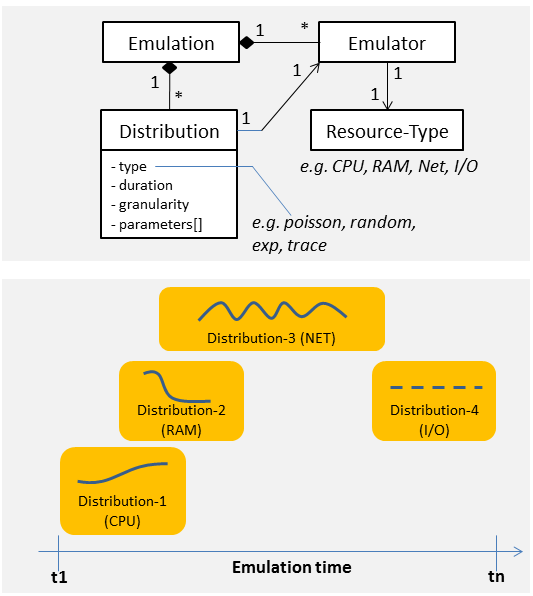
\includegraphics{emulation2.png}
\end{figure}
\end{quote}


\subsection{Getting Started}
\label{COCOMA/02_how_to_use_it:getting-started}\label{COCOMA/02_how_to_use_it::doc}
COCOMA is installed in \emph{``/usr/share/pyshared/cocoma''}. In this section we provide information about the components that have to be running in order to fully use the framework, and how can a user interact with it.


\subsubsection{Starting Components}
\label{COCOMA/02_how_to_use_it:starting-components}
The two main components of COCOMA are:
\begin{itemize}
\item {} 
Scheduler daemon (mandatory, needs to be the first started)

\item {} 
API Daemon (optional, if the REST API functionality is required)

\end{itemize}

The \textbf{Scheduler daemon} - runs in the background and executes workload with differential parameters at the time defined in the emulation properties.
To check if the scheduler is running use the following:

\begin{Verbatim}[commandchars=\\\{\}]
\PYG{n+nv}{\PYGZdl{} }ccmsh \PYGZhy{}\PYGZhy{}show scheduler
\end{Verbatim}

To start the scheduler on a specific network interface and port, use the command:

\begin{Verbatim}[commandchars=\\\{\}]
\PYG{n+nv}{\PYGZdl{} }ccmsh \PYGZhy{}\PYGZhy{}start scheduler eth1 55555
\end{Verbatim}

If the network interface and port are omitted, the default values are respectively \emph{eth0} adn \emph{51889}

If more detailed output information is needed, the \emph{Scheduler} can also be started in \emph{DEBUG} mode:

\begin{Verbatim}[commandchars=\\\{\}]
\PYG{n+nv}{\PYGZdl{} }ccmsh \PYGZhy{}\PYGZhy{}start scheduler eth1 55555 debug
\end{Verbatim}

The \textbf{API daemon} - provides the RESTfull web API, which exposes COCOMA resources to be used over the network. It follows the same command structure as the Scheduler.
To check if the scheduler is running use the following:

\begin{Verbatim}[commandchars=\\\{\}]
\PYG{n+nv}{\PYGZdl{} }ccmsh \PYGZhy{}\PYGZhy{}show api
\end{Verbatim}

To start the api on a specific network interface and port, use the command:

\begin{Verbatim}[commandchars=\\\{\}]
\PYG{n+nv}{\PYGZdl{} }ccmsh \PYGZhy{}\PYGZhy{}start api eth2 77777
\end{Verbatim}

If the network interface and port are omitted, the default values are respectively \emph{eth0} and \emph{5050}

The log level is the same specified for the \emph{Scheduler}.


\subsubsection{CLI}
\label{COCOMA/02_how_to_use_it:cli}
The COCOMA CLI is called \emph{ccmsh}, and provides the following options:
\index{ccmsh command line option!-h, --help}\index{-h, --help!ccmsh command line option}

\begin{fulllineitems}
\phantomsection\label{COCOMA/02_how_to_use_it:cmdoption-ccmsh-h}\pysigline{\bfcode{-h}\code{}\code{,~}\bfcode{--help}\code{}}
Display help information of the available options

\end{fulllineitems}

\index{ccmsh command line option!-v, --version}\index{-v, --version!ccmsh command line option}

\begin{fulllineitems}
\phantomsection\label{COCOMA/02_how_to_use_it:cmdoption-ccmsh-v}\pysigline{\bfcode{-v}\code{}\code{,~}\bfcode{--version}\code{}}
Display installed version information of COCOMA

\end{fulllineitems}

\index{ccmsh command line option!-l, --list \textless{}emulation name\textgreater{}}\index{-l, --list \textless{}emulation name\textgreater{}!ccmsh command line option}

\begin{fulllineitems}
\phantomsection\label{COCOMA/02_how_to_use_it:cmdoption-ccmsh-l}\pysigline{\bfcode{-l}\code{}\code{,~}\bfcode{--list}\code{~\textless{}emulation~name\textgreater{}}}
Display list of all emulations that are scheduled or already finished. If emulation name is provided then it lists information for that specific emulation

\end{fulllineitems}

\index{ccmsh command line option!-r, --results \textless{}emulation name\textgreater{}}\index{-r, --results \textless{}emulation name\textgreater{}!ccmsh command line option}

\begin{fulllineitems}
\phantomsection\label{COCOMA/02_how_to_use_it:cmdoption-ccmsh-r}\pysigline{\bfcode{-r}\code{}\code{,~}\bfcode{--results}\code{~\textless{}emulation~name\textgreater{}}}
Display list of results of all emulations that are scheduled or already finished. If emulation name is provided, then it lists information for that specific emulation

\end{fulllineitems}

\index{ccmsh command line option!-j, --list-jobs}\index{-j, --list-jobs!ccmsh command line option}

\begin{fulllineitems}
\phantomsection\label{COCOMA/02_how_to_use_it:cmdoption-ccmsh-j}\pysigline{\bfcode{-j}\code{}\code{,~}\bfcode{--list-jobs}\code{}}
Queries the scheduler for the list of jobs that have to be executed. For each one, it gives the job name and the planned execution time

\end{fulllineitems}

\index{ccmsh command line option!-i, --dist \textless{}distribution name\textgreater{}}\index{-i, --dist \textless{}distribution name\textgreater{}!ccmsh command line option}

\begin{fulllineitems}
\phantomsection\label{COCOMA/02_how_to_use_it:cmdoption-ccmsh-i}\pysigline{\bfcode{-i}\code{}\code{,~}\bfcode{--dist}\code{~\textless{}distribution~name\textgreater{}}}
Scans the \emph{``/usr/share/pyshared/cocoma/distributions''} folder and displays all available distribution modules. If a distribution name is provided, then it shows the help information for that specific distribution

\end{fulllineitems}

\index{ccmsh command line option!-e, --emu \textless{}emulator name\textgreater{}}\index{-e, --emu \textless{}emulator name\textgreater{}!ccmsh command line option}

\begin{fulllineitems}
\phantomsection\label{COCOMA/02_how_to_use_it:cmdoption-ccmsh-e}\pysigline{\bfcode{-e}\code{}\code{,~}\bfcode{--emu}\code{~\textless{}emulator~name\textgreater{}}}
Scans the \emph{``/usr/share/pyshared/cocoma/emulators''} folder and displays all available emulator wrapper modules. If an emulator name is provided, then it shows the help information for that specific emulator wrapper

\end{fulllineitems}

\index{ccmsh command line option!-x, --xml \textless{}file name\textgreater{}}\index{-x, --xml \textless{}file name\textgreater{}!ccmsh command line option}

\begin{fulllineitems}
\phantomsection\label{COCOMA/02_how_to_use_it:cmdoption-ccmsh-x}\pysigline{\bfcode{-x}\code{}\code{,~}\bfcode{--xml}\code{~\textless{}file~name\textgreater{}}}
It create and emulation based on the local XML

\end{fulllineitems}

\index{ccmsh command line option!-n, --now (used with -x option only)}\index{-n, --now (used with -x option only)!ccmsh command line option}

\begin{fulllineitems}
\phantomsection\label{COCOMA/02_how_to_use_it:cmdoption-ccmsh-n}\pysigline{\bfcode{-n}\code{}\code{,~}\bfcode{--now}\code{~(used~with~-x~option~only)}}
Override any start date in the local XML emulation file without modifying the file, i.e. \code{ccmsh -x \textless{}file name\textgreater{} -n}

\end{fulllineitems}

\index{ccmsh command line option!-d, --delete \textless{}emulation name\textgreater{}}\index{-d, --delete \textless{}emulation name\textgreater{}!ccmsh command line option}

\begin{fulllineitems}
\phantomsection\label{COCOMA/02_how_to_use_it:cmdoption-ccmsh-d}\pysigline{\bfcode{-d}\code{}\code{,~}\bfcode{--delete}\code{~\textless{}emulation~name\textgreater{}}}
Deletes a specific emulation from the database

\end{fulllineitems}

\index{ccmsh command line option!-p, --purge}\index{-p, --purge!ccmsh command line option}

\begin{fulllineitems}
\phantomsection\label{COCOMA/02_how_to_use_it:cmdoption-ccmsh-p}\pysigline{\bfcode{-p}\code{}\code{,~}\bfcode{--purge}\code{}}
Remove all DB entries, all scheduled jobs

\end{fulllineitems}

\index{ccmsh command line option!--start \textless{}api interface port\textgreater{}, \textless{}scheduler interface port\textgreater{}}\index{--start \textless{}api interface port\textgreater{}, \textless{}scheduler interface port\textgreater{}!ccmsh command line option}

\begin{fulllineitems}
\phantomsection\label{COCOMA/02_how_to_use_it:cmdoption-ccmsh--start}\pysigline{\bfcode{--start}\code{~\textless{}api~interface~port\textgreater{},~\textless{}scheduler~interface~port\textgreater{}}}
Start Scheduler or API daemon by specifying network interface and port number i.e. \code{ccmsh -{-}start api eth0 2020} or \code{ccmsh -{-}start scheduler eth0 3030}. By default if the network interface is not specified, the Scheduler daemon will run on \emph{eth0} and \emph{51889}, and the API daemon will run on \emph{eth0} and \emph{5050}.

\end{fulllineitems}

\index{ccmsh command line option!--stop \textless{}api\textgreater{}, \textless{}scheduler\textgreater{}}\index{--stop \textless{}api\textgreater{}, \textless{}scheduler\textgreater{}!ccmsh command line option}

\begin{fulllineitems}
\phantomsection\label{COCOMA/02_how_to_use_it:cmdoption-ccmsh--stop}\pysigline{\bfcode{--stop}\code{~\textless{}api\textgreater{},~\textless{}scheduler\textgreater{}}}
Stop Scheduler or API daemon

\end{fulllineitems}

\index{ccmsh command line option!--show \textless{}api\textgreater{}, \textless{}scheduler\textgreater{}}\index{--show \textless{}api\textgreater{}, \textless{}scheduler\textgreater{}!ccmsh command line option}

\begin{fulllineitems}
\phantomsection\label{COCOMA/02_how_to_use_it:cmdoption-ccmsh--show}\pysigline{\bfcode{--show}\code{~\textless{}api\textgreater{},~\textless{}scheduler\textgreater{}}}
Show OS information on Scheduler or API daemon, displays PID numbers

\end{fulllineitems}



\subsubsection{REST API}
\label{COCOMA/02_how_to_use_it:rest-api}

\paragraph{Index}
\label{COCOMA/02_how_to_use_it:index}
The API URIs summary list is as follow:

\begin{Verbatim}[commandchars=\\\{\}]
* /
* /emulations
* /emulations/\PYGZob{}name\PYGZcb{}
* /distributions
* /distributions/\PYGZob{}name\PYGZcb{}
* /emulators
* /emulators/\PYGZob{}name\PYGZcb{}
* /results
* /results/\PYGZob{}name\PYGZcb{}
* /tests
* /tests/\PYGZob{}name\PYGZcb{}
* /logs
* /logs/system
* /logs/emulations
* /logs/emulations/\PYGZob{}name\PYGZcb{}
\end{Verbatim}


\paragraph{Description}
\label{COCOMA/02_how_to_use_it:description}
\code{http:method:: GET /}
\begin{quote}

The \textbf{root} returns a \emph{collection} of all the available resources. Example of a XML response:

\begin{Verbatim}[commandchars=\\\{\}]
\PYG{c+cp}{\PYGZlt{}?xml version=\PYGZdq{}1.0\PYGZdq{} ?\PYGZgt{}}
\PYG{n+nt}{\PYGZlt{}root} \PYG{n+na}{href=}\PYG{l+s}{\PYGZdq{}/\PYGZdq{}}\PYG{n+nt}{\PYGZgt{}}
        \PYG{n+nt}{\PYGZlt{}version}\PYG{n+nt}{\PYGZgt{}}0.1.1\PYG{n+nt}{\PYGZlt{}/version\PYGZgt{}}
        \PYG{n+nt}{\PYGZlt{}timestamp}\PYG{n+nt}{\PYGZgt{}}1365518303.44\PYG{n+nt}{\PYGZlt{}/timestamp\PYGZgt{}}
        \PYG{n+nt}{\PYGZlt{}link} \PYG{n+na}{href=}\PYG{l+s}{\PYGZdq{}/emulations\PYGZdq{}} \PYG{n+na}{rel=}\PYG{l+s}{\PYGZdq{}emulations\PYGZdq{}} \PYG{n+na}{type=}\PYG{l+s}{\PYGZdq{}application/vnd.bonfire+xml\PYGZdq{}}\PYG{n+nt}{/\PYGZgt{}}
        \PYG{n+nt}{\PYGZlt{}link} \PYG{n+na}{href=}\PYG{l+s}{\PYGZdq{}/emulators\PYGZdq{}} \PYG{n+na}{rel=}\PYG{l+s}{\PYGZdq{}emulators\PYGZdq{}} \PYG{n+na}{type=}\PYG{l+s}{\PYGZdq{}application/vnd.bonfire+xml\PYGZdq{}}\PYG{n+nt}{/\PYGZgt{}}
        \PYG{n+nt}{\PYGZlt{}link} \PYG{n+na}{href=}\PYG{l+s}{\PYGZdq{}/distributions\PYGZdq{}} \PYG{n+na}{rel=}\PYG{l+s}{\PYGZdq{}distributions\PYGZdq{}} \PYG{n+na}{type=}\PYG{l+s}{\PYGZdq{}application/vnd.bonfire+xml\PYGZdq{}}\PYG{n+nt}{/\PYGZgt{}}
        \PYG{n+nt}{\PYGZlt{}link} \PYG{n+na}{href=}\PYG{l+s}{\PYGZdq{}/tests\PYGZdq{}} \PYG{n+na}{rel=}\PYG{l+s}{\PYGZdq{}tests\PYGZdq{}} \PYG{n+na}{type=}\PYG{l+s}{\PYGZdq{}application/vnd.bonfire+xml\PYGZdq{}}\PYG{n+nt}{/\PYGZgt{}}
        \PYG{n+nt}{\PYGZlt{}link} \PYG{n+na}{href=}\PYG{l+s}{\PYGZdq{}/results\PYGZdq{}} \PYG{n+na}{rel=}\PYG{l+s}{\PYGZdq{}results\PYGZdq{}} \PYG{n+na}{type=}\PYG{l+s}{\PYGZdq{}application/vnd.bonfire+xml\PYGZdq{}}\PYG{n+nt}{/\PYGZgt{}}
        \PYG{n+nt}{\PYGZlt{}link} \PYG{n+na}{href=}\PYG{l+s}{\PYGZdq{}/logs\PYGZdq{}} \PYG{n+na}{rel=}\PYG{l+s}{\PYGZdq{}logs\PYGZdq{}} \PYG{n+na}{type=}\PYG{l+s}{\PYGZdq{}application/vnd.bonfire+xml\PYGZdq{}}\PYG{n+nt}{/\PYGZgt{}}
\PYG{n+nt}{\PYGZlt{}/root\PYGZgt{}}
\end{Verbatim}
\end{quote}

\code{http:method:: GET /emulations}
\begin{quote}

The \textbf{emulations} returns a \emph{collection} of all the available emulation resources. Example of a XML response:

\begin{Verbatim}[commandchars=\\\{\}]
\PYG{c+cp}{\PYGZlt{}?xml version=\PYGZdq{}1.0\PYGZdq{} ?\PYGZgt{}}
\PYG{n+nt}{\PYGZlt{}collection} \PYG{n+na}{href=}\PYG{l+s}{\PYGZdq{}/emulations\PYGZdq{}} \PYG{n+na}{xmlns=}\PYG{l+s}{\PYGZdq{}http://127.0.0.1/cocoma\PYGZdq{}}\PYG{n+nt}{\PYGZgt{}}
        \PYG{n+nt}{\PYGZlt{}items} \PYG{n+na}{offset=}\PYG{l+s}{\PYGZdq{}0\PYGZdq{}} \PYG{n+na}{total=}\PYG{l+s}{\PYGZdq{}3\PYGZdq{}}\PYG{n+nt}{\PYGZgt{}}
                \PYG{n+nt}{\PYGZlt{}emulation} \PYG{n+na}{href=}\PYG{l+s}{\PYGZdq{}/emulations/1\PYGZhy{}Emu\PYGZhy{}CPU\PYGZhy{}RAM\PYGZhy{}IO\PYGZdq{}} \PYG{n+na}{id=}\PYG{l+s}{\PYGZdq{}1\PYGZdq{}} \PYG{n+na}{name=}\PYG{l+s}{\PYGZdq{}1\PYGZhy{}Emu\PYGZhy{}CPU\PYGZhy{}RAM\PYGZhy{}IO\PYGZdq{}} \PYG{n+na}{state=}\PYG{l+s}{\PYGZdq{}inactive\PYGZdq{}}\PYG{n+nt}{/\PYGZgt{}}
                \PYG{n+nt}{\PYGZlt{}emulation} \PYG{n+na}{href=}\PYG{l+s}{\PYGZdq{}/emulations/2\PYGZhy{}CPU\PYGZus{}EMU\PYGZdq{}} \PYG{n+na}{id=}\PYG{l+s}{\PYGZdq{}2\PYGZdq{}} \PYG{n+na}{name=}\PYG{l+s}{\PYGZdq{}2\PYGZhy{}CPU\PYGZus{}EMU\PYGZdq{}} \PYG{n+na}{state=}\PYG{l+s}{\PYGZdq{}inactive\PYGZdq{}}\PYG{n+nt}{/\PYGZgt{}}
                \PYG{n+nt}{\PYGZlt{}emulation} \PYG{n+na}{href=}\PYG{l+s}{\PYGZdq{}/emulations/3\PYGZhy{}CPU\PYGZus{}EMU\PYGZdq{}} \PYG{n+na}{id=}\PYG{l+s}{\PYGZdq{}3\PYGZdq{}} \PYG{n+na}{name=}\PYG{l+s}{\PYGZdq{}3\PYGZhy{}CPU\PYGZus{}EMU\PYGZdq{}} \PYG{n+na}{state=}\PYG{l+s}{\PYGZdq{}inactive\PYGZdq{}}\PYG{n+nt}{/\PYGZgt{}}
        \PYG{n+nt}{\PYGZlt{}/items\PYGZgt{}}
        \PYG{n+nt}{\PYGZlt{}link} \PYG{n+na}{href=}\PYG{l+s}{\PYGZdq{}/\PYGZdq{}} \PYG{n+na}{rel=}\PYG{l+s}{\PYGZdq{}parent\PYGZdq{}} \PYG{n+na}{type=}\PYG{l+s}{\PYGZdq{}application/vnd.bonfire+xml\PYGZdq{}}\PYG{n+nt}{/\PYGZgt{}}
\PYG{n+nt}{\PYGZlt{}/collection\PYGZgt{}}
\end{Verbatim}
\end{quote}

\code{http:method:: GET /emulations/\{name\}}
\begin{quote}

Displays information about emulation by name. The returned \emph{200-OK} XML is:

\begin{Verbatim}[commandchars=\\\{\}]
\PYG{c+cp}{\PYGZlt{}?xml version=\PYGZdq{}1.0\PYGZdq{} ?\PYGZgt{}}
\PYG{n+nt}{\PYGZlt{}emulation} \PYG{n+na}{href=}\PYG{l+s}{\PYGZdq{}/emulations/1\PYGZhy{}Emu\PYGZhy{}CPU\PYGZhy{}RAM\PYGZhy{}IO\PYGZdq{}} \PYG{n+na}{xmlns=}\PYG{l+s}{\PYGZdq{}http://127.0.0.1/cocoma\PYGZdq{}}\PYG{n+nt}{\PYGZgt{}}
        \PYG{n+nt}{\PYGZlt{}id}\PYG{n+nt}{\PYGZgt{}}1\PYG{n+nt}{\PYGZlt{}/id\PYGZgt{}}
        \PYG{n+nt}{\PYGZlt{}emulationName}\PYG{n+nt}{\PYGZgt{}}1\PYGZhy{}Emu\PYGZhy{}CPU\PYGZhy{}RAM\PYGZhy{}IO\PYG{n+nt}{\PYGZlt{}/emulationName\PYGZgt{}}
        \PYG{n+nt}{\PYGZlt{}emulationType}\PYG{n+nt}{\PYGZgt{}}mix\PYG{n+nt}{\PYGZlt{}/emulationType\PYGZgt{}}
        \PYG{n+nt}{\PYGZlt{}resourceType}\PYG{n+nt}{\PYGZgt{}}mix\PYG{n+nt}{\PYGZlt{}/resourceType\PYGZgt{}}
        \PYG{n+nt}{\PYGZlt{}emuStartTime}\PYG{n+nt}{\PYGZgt{}}2013\PYGZhy{}04\PYGZhy{}09T13:00:01\PYG{n+nt}{\PYGZlt{}/emuStartTime\PYGZgt{}}
        \PYG{n+nt}{\PYGZlt{}emuStopTime}\PYG{n+nt}{\PYGZgt{}}180\PYG{n+nt}{\PYGZlt{}/emuStopTime\PYGZgt{}}
        \PYG{n+nt}{\PYGZlt{}scheduledJobs}\PYG{n+nt}{\PYGZgt{}}
                \PYG{n+nt}{\PYGZlt{}jobsempty}\PYG{n+nt}{\PYGZgt{}}No jobs are scheduled\PYG{n+nt}{\PYGZlt{}/jobsempty\PYGZgt{}}
        \PYG{n+nt}{\PYGZlt{}/scheduledJobs\PYGZgt{}}
        \PYG{n+nt}{\PYGZlt{}distributions} \PYG{n+na}{ID=}\PYG{l+s}{\PYGZdq{}1\PYGZdq{}} \PYG{n+na}{name=}\PYG{l+s}{\PYGZdq{}Distro1\PYGZdq{}}\PYG{n+nt}{\PYGZgt{}}
                \PYG{n+nt}{\PYGZlt{}startTime}\PYG{n+nt}{\PYGZgt{}}5\PYG{n+nt}{\PYGZlt{}/startTime\PYGZgt{}}
                \PYG{n+nt}{\PYGZlt{}granularity}\PYG{n+nt}{\PYGZgt{}}3\PYG{n+nt}{\PYGZlt{}/granularity\PYGZgt{}}
                \PYG{n+nt}{\PYGZlt{}duration}\PYG{n+nt}{\PYGZgt{}}30\PYG{n+nt}{\PYGZlt{}/duration\PYGZgt{}}
                \PYG{n+nt}{\PYGZlt{}startload}\PYG{n+nt}{\PYGZgt{}}10\PYG{n+nt}{\PYGZlt{}/startload\PYGZgt{}}
                \PYG{n+nt}{\PYGZlt{}stopload}\PYG{n+nt}{\PYGZgt{}}90\PYG{n+nt}{\PYGZlt{}/stopload\PYGZgt{}}
        \PYG{n+nt}{\PYGZlt{}/distributions\PYGZgt{}}
        \PYG{n+nt}{\PYGZlt{}distributions} \PYG{n+na}{ID=}\PYG{l+s}{\PYGZdq{}2\PYGZdq{}} \PYG{n+na}{name=}\PYG{l+s}{\PYGZdq{}Distro2\PYGZdq{}}\PYG{n+nt}{\PYGZgt{}}
                \PYG{n+nt}{\PYGZlt{}startTime}\PYG{n+nt}{\PYGZgt{}}5\PYG{n+nt}{\PYGZlt{}/startTime\PYGZgt{}}
                \PYG{n+nt}{\PYGZlt{}granularity}\PYG{n+nt}{\PYGZgt{}}3\PYG{n+nt}{\PYGZlt{}/granularity\PYGZgt{}}
                \PYG{n+nt}{\PYGZlt{}duration}\PYG{n+nt}{\PYGZgt{}}30\PYG{n+nt}{\PYGZlt{}/duration\PYGZgt{}}
                \PYG{n+nt}{\PYGZlt{}startload}\PYG{n+nt}{\PYGZgt{}}10\PYG{n+nt}{\PYGZlt{}/startload\PYGZgt{}}
                \PYG{n+nt}{\PYGZlt{}stopload}\PYG{n+nt}{\PYGZgt{}}90\PYG{n+nt}{\PYGZlt{}/stopload\PYGZgt{}}
        \PYG{n+nt}{\PYGZlt{}/distributions\PYGZgt{}}
        \PYG{n+nt}{\PYGZlt{}link} \PYG{n+na}{href=}\PYG{l+s}{\PYGZdq{}/\PYGZdq{}} \PYG{n+na}{rel=}\PYG{l+s}{\PYGZdq{}parent\PYGZdq{}} \PYG{n+na}{type=}\PYG{l+s}{\PYGZdq{}application/vnd.bonfire+xml\PYGZdq{}}\PYG{n+nt}{/\PYGZgt{}}
        \PYG{n+nt}{\PYGZlt{}link} \PYG{n+na}{href=}\PYG{l+s}{\PYGZdq{}/emulations\PYGZdq{}} \PYG{n+na}{rel=}\PYG{l+s}{\PYGZdq{}parent\PYGZdq{}} \PYG{n+na}{type=}\PYG{l+s}{\PYGZdq{}application/vnd.bonfire+xml\PYGZdq{}}\PYG{n+nt}{/\PYGZgt{}}
\PYG{n+nt}{\PYGZlt{}/emulation\PYGZgt{}}
\end{Verbatim}

The returned \emph{404 – Not Found} XML is:

\begin{Verbatim}[commandchars=\\\{\}]
\PYG{n+nt}{\PYGZlt{}error}\PYG{n+nt}{\PYGZgt{}}Emulation Name: 1\PYGZhy{}Emu\PYGZhy{}CPU\PYGZhy{}RAM\PYGZhy{}IO1 not found. Error:too many values to unpack\PYG{n+nt}{\PYGZlt{}/error\PYGZgt{}}
\end{Verbatim}
\end{quote}

\code{http:method:: POST /emulations}
\begin{quote}

\begin{Verbatim}[commandchars=\\\{\}]
:param string XML: Emulation parameters defined via XML as shown in the examples section.
\end{Verbatim}

The returned \emph{201-Created} XML:

\begin{Verbatim}[commandchars=\\\{\}]
\PYG{c+cp}{\PYGZlt{}?xml version=\PYGZdq{}1.0\PYGZdq{} ?\PYGZgt{}}
\PYG{n+nt}{\PYGZlt{}emulation} \PYG{n+na}{href=}\PYG{l+s}{\PYGZdq{}/emulations/4\PYGZhy{}CPU\PYGZus{}EMU\PYGZdq{}} \PYG{n+na}{xmlns=}\PYG{l+s}{\PYGZdq{}http://127.0.0.1/cocoma\PYGZdq{}}\PYG{n+nt}{\PYGZgt{}}
        \PYG{n+nt}{\PYGZlt{}ID}\PYG{n+nt}{\PYGZgt{}}4\PYGZhy{}CPU\PYGZus{}EMU\PYG{n+nt}{\PYGZlt{}/ID\PYGZgt{}}
        \PYG{n+nt}{\PYGZlt{}EmuNotes}\PYG{n+nt}{\PYGZgt{}}OK\PYG{n+nt}{\PYGZlt{}/EmuNotes\PYGZgt{}}
        \PYG{n+nt}{\PYGZlt{}DistroNotes}\PYG{n+nt}{\PYGZgt{}}OK\PYG{n+nt}{\PYGZlt{}/DistroNotes\PYGZgt{}}
        \PYG{n+nt}{\PYGZlt{}link} \PYG{n+na}{href=}\PYG{l+s}{\PYGZdq{}/\PYGZdq{}} \PYG{n+na}{rel=}\PYG{l+s}{\PYGZdq{}parent\PYGZdq{}} \PYG{n+na}{type=}\PYG{l+s}{\PYGZdq{}application/vnd.bonfire+xml\PYGZdq{}}\PYG{n+nt}{/\PYGZgt{}}
        \PYG{n+nt}{\PYGZlt{}link} \PYG{n+na}{href=}\PYG{l+s}{\PYGZdq{}/emulations\PYGZdq{}} \PYG{n+na}{rel=}\PYG{l+s}{\PYGZdq{}parent\PYGZdq{}} \PYG{n+na}{type=}\PYG{l+s}{\PYGZdq{}application/vnd.bonfire+xml\PYGZdq{}}\PYG{n+nt}{/\PYGZgt{}}
\PYG{n+nt}{\PYGZlt{}/emulation\PYGZgt{}}
\end{Verbatim}

The returned \emph{400 – Bad Request} XML:

\begin{Verbatim}[commandchars=\\\{\}]
\PYG{c+cp}{\PYGZlt{}?xml version=\PYGZdq{}1.0\PYGZdq{} ?\PYGZgt{}}
\PYG{n+nt}{\PYGZlt{}error}\PYG{n+nt}{\PYGZgt{}}XML is not well formed Error: syntax error: line 1, column 0\PYG{n+nt}{\PYGZlt{}/error\PYGZgt{}}
\end{Verbatim}
\end{quote}

\code{http:method:: GET /emulators}
\begin{quote}

Displays emulators list. The returned \emph{200- OK} XML:

\begin{Verbatim}[commandchars=\\\{\}]
\PYG{c+cp}{\PYGZlt{}?xml version=\PYGZdq{}1.0\PYGZdq{} ?\PYGZgt{}}
\PYG{n+nt}{\PYGZlt{}collection} \PYG{n+na}{href=}\PYG{l+s}{\PYGZdq{}/emulators\PYGZdq{}} \PYG{n+na}{xmlns=}\PYG{l+s}{\PYGZdq{}http://127.0.0.1/cocoma\PYGZdq{}}\PYG{n+nt}{\PYGZgt{}}
        \PYG{n+nt}{\PYGZlt{}items} \PYG{n+na}{offset=}\PYG{l+s}{\PYGZdq{}0\PYGZdq{}} \PYG{n+na}{total=}\PYG{l+s}{\PYGZdq{}3\PYGZdq{}}\PYG{n+nt}{\PYGZgt{}}
                \PYG{n+nt}{\PYGZlt{}emulator} \PYG{n+na}{href=}\PYG{l+s}{\PYGZdq{}/emulators/lookbusy\PYGZdq{}} \PYG{n+na}{name=}\PYG{l+s}{\PYGZdq{}lookbusy\PYGZdq{}}\PYG{n+nt}{/\PYGZgt{}}
                \PYG{n+nt}{\PYGZlt{}emulator} \PYG{n+na}{href=}\PYG{l+s}{\PYGZdq{}/emulators/stressapptest\PYGZdq{}} \PYG{n+na}{name=}\PYG{l+s}{\PYGZdq{}stressapptest\PYGZdq{}}\PYG{n+nt}{/\PYGZgt{}}
                \PYG{n+nt}{\PYGZlt{}emulator} \PYG{n+na}{href=}\PYG{l+s}{\PYGZdq{}/emulators/iperf\PYGZdq{}} \PYG{n+na}{name=}\PYG{l+s}{\PYGZdq{}iperf\PYGZdq{}}\PYG{n+nt}{/\PYGZgt{}}
        \PYG{n+nt}{\PYGZlt{}/items\PYGZgt{}}
        \PYG{n+nt}{\PYGZlt{}link} \PYG{n+na}{href=}\PYG{l+s}{\PYGZdq{}/\PYGZdq{}} \PYG{n+na}{rel=}\PYG{l+s}{\PYGZdq{}parent\PYGZdq{}} \PYG{n+na}{type=}\PYG{l+s}{\PYGZdq{}application/vnd.bonfire+xml\PYGZdq{}}\PYG{n+nt}{/\PYGZgt{}}
\PYG{n+nt}{\PYGZlt{}/collection\PYGZgt{}}
\end{Verbatim}
\end{quote}

\code{http:method:: GET /emulators/\{name\}}
\begin{quote}
\begin{quote}

\begin{Verbatim}[commandchars=\\\{\}]
:arg name: Name of emulator that you want to get more info
\end{Verbatim}

Displays information about emulator by name. The returned \emph{200- OK} XML:

\begin{Verbatim}[commandchars=\\\{\}]
\end{Verbatim}
\end{quote}

\textless{}?xml version=''1.0'' ?\textgreater{}
\textless{}emulator href=''/emulators/lookbusy'' xmlns=''\href{http://127.0.0.1/cocoma}{http://127.0.0.1/cocoma}``\textgreater{}
\begin{quote}
\begin{description}
\item[{\textless{}info\textgreater{}}] \leavevmode
\textless{}help\textgreater{}
Emulator lookbusy can be used for following resources:
1)Loads CPU with parameters:
\begin{quote}

ncpus - Number of CPUs to keep busy (default: autodetected)
\end{quote}
\begin{description}
\item[{2)Loads Memory(MEM) with parameters:}] \leavevmode
memSleep - Time to sleep between iterations, in usec (default 1000)

\item[{3)Changing size of files to use during IO with parameters:}] \leavevmode
ioBlockSize - Size of blocks to use for I/O in MB
ioSleep - Time to sleep between iterations, in msec (default 100)

\end{description}

XML block example:
\&lt;emulator-params\&gt;
\begin{quote}

\&lt;resourceType\&gt;CPU\&lt;/resourceType\&gt;
\&lt;ncpus\&gt;0\&lt;/ncpus\&gt;
\end{quote}

\&lt;/emulator-params\&gt;

\textless{}/help\textgreater{}
\textless{}resources\textgreater{}
\begin{quote}
\begin{description}
\item[{\textless{}cpu\textgreater{}}] \leavevmode\begin{description}
\item[{\textless{}ncpus\textgreater{}}] \leavevmode
\textless{}upperBound\textgreater{}100\textless{}/upperBound\textgreater{}
\textless{}lowerBound\textgreater{}100\textless{}/lowerBound\textgreater{}

\end{description}

\textless{}/ncpus\textgreater{}

\end{description}

\textless{}/cpu\textgreater{}
\textless{}io\textgreater{}
\begin{quote}
\begin{description}
\item[{\textless{}iosleep\textgreater{}}] \leavevmode
\textless{}upperBound\textgreater{}999999999\textless{}/upperBound\textgreater{}
\textless{}lowerBound\textgreater{}999999999\textless{}/lowerBound\textgreater{}

\end{description}

\textless{}/iosleep\textgreater{}
\textless{}ioblocksize\textgreater{}
\begin{quote}

\textless{}upperBound\textgreater{}9999999\textless{}/upperBound\textgreater{}
\textless{}lowerBound\textgreater{}9999999\textless{}/lowerBound\textgreater{}
\end{quote}

\textless{}/ioblocksize\textgreater{}
\end{quote}

\textless{}/io\textgreater{}
\textless{}mem\textgreater{}
\begin{quote}
\begin{description}
\item[{\textless{}memsleep\textgreater{}}] \leavevmode
\textless{}upperBound\textgreater{}999999999\textless{}/upperBound\textgreater{}
\textless{}lowerBound\textgreater{}999999999\textless{}/lowerBound\textgreater{}

\end{description}

\textless{}/memsleep\textgreater{}
\end{quote}

\textless{}/mem\textgreater{}
\end{quote}

\textless{}/resources\textgreater{}

\end{description}

\textless{}/info\textgreater{}
\textless{}link href=''/'' rel=''parent'' type=''application/vnd.bonfire+xml''/\textgreater{}
\textless{}link href=''/emulators'' rel=''parent'' type=''application/vnd.bonfire+xml''/\textgreater{}
\end{quote}

\textless{}/emulator\textgreater{}
\end{quote}

\code{http:method:: GET /distributions}
\begin{quote}

Displays distributions list. The returned \emph{200- OK} XML:

\begin{Verbatim}[commandchars=\\\{\}]
\PYG{c+cp}{\PYGZlt{}?xml version=\PYGZdq{}1.0\PYGZdq{} ?\PYGZgt{}}
\PYG{n+nt}{\PYGZlt{}collection} \PYG{n+na}{href=}\PYG{l+s}{\PYGZdq{}/distributions\PYGZdq{}} \PYG{n+na}{xmlns=}\PYG{l+s}{\PYGZdq{}http://127.0.0.1/cocoma\PYGZdq{}}\PYG{n+nt}{\PYGZgt{}}
        \PYG{n+nt}{\PYGZlt{}items} \PYG{n+na}{offset=}\PYG{l+s}{\PYGZdq{}0\PYGZdq{}} \PYG{n+na}{total=}\PYG{l+s}{\PYGZdq{}3\PYGZdq{}}\PYG{n+nt}{\PYGZgt{}}
                \PYG{n+nt}{\PYGZlt{}distribution} \PYG{n+na}{href=}\PYG{l+s}{\PYGZdq{}/distributions/linear\PYGZdq{}} \PYG{n+na}{name=}\PYG{l+s}{\PYGZdq{}linear\PYGZdq{}}\PYG{n+nt}{/\PYGZgt{}}
                \PYG{n+nt}{\PYGZlt{}distribution} \PYG{n+na}{href=}\PYG{l+s}{\PYGZdq{}/distributions/linear\PYGZus{}incr\PYGZdq{}} \PYG{n+na}{name=}\PYG{l+s}{\PYGZdq{}linear\PYGZus{}incr\PYGZdq{}}\PYG{n+nt}{/\PYGZgt{}}
                \PYG{n+nt}{\PYGZlt{}distribution} \PYG{n+na}{href=}\PYG{l+s}{\PYGZdq{}/distributions/trapezoidal\PYGZdq{}} \PYG{n+na}{name=}\PYG{l+s}{\PYGZdq{}trapezoidal\PYGZdq{}}\PYG{n+nt}{/\PYGZgt{}}
        \PYG{n+nt}{\PYGZlt{}/items\PYGZgt{}}
        \PYG{n+nt}{\PYGZlt{}link} \PYG{n+na}{href=}\PYG{l+s}{\PYGZdq{}/\PYGZdq{}} \PYG{n+na}{rel=}\PYG{l+s}{\PYGZdq{}parent\PYGZdq{}} \PYG{n+na}{type=}\PYG{l+s}{\PYGZdq{}application/vnd.bonfire+xml\PYGZdq{}}\PYG{n+nt}{/\PYGZgt{}}
\PYG{n+nt}{\PYGZlt{}/collection\PYGZgt{}}
\end{Verbatim}
\end{quote}

\code{http:method:: GET /distributions/\{name\}}
\begin{quote}

\begin{Verbatim}[commandchars=\\\{\}]
:arg name: Name of distributions that you want to get more info
\end{Verbatim}

Displays information about distributions by name. The returned \emph{200- OK} XML:

\begin{Verbatim}[commandchars=\\\{\}]
\PYG{c+cp}{\PYGZlt{}?xml version=\PYGZdq{}1.0\PYGZdq{} ?\PYGZgt{}}
\PYG{n+nt}{\PYGZlt{}distribution} \PYG{n+na}{href=}\PYG{l+s}{\PYGZdq{}/distributions/linear\PYGZdq{}} \PYG{n+na}{xmlns=}\PYG{l+s}{\PYGZdq{}http://127.0.0.1/cocoma\PYGZdq{}}\PYG{n+nt}{\PYGZgt{}}
        \PYG{n+nt}{\PYGZlt{}info}\PYG{n+nt}{\PYGZgt{}}Linear distribution takes in start and stop load parameters and gradually increasing resource workload. Can be used with CPU,MEM,IO,NET resource types.\PYG{n+nt}{\PYGZlt{}/info\PYGZgt{}}
        \PYG{n+nt}{\PYGZlt{}link} \PYG{n+na}{href=}\PYG{l+s}{\PYGZdq{}/\PYGZdq{}} \PYG{n+na}{rel=}\PYG{l+s}{\PYGZdq{}parent\PYGZdq{}} \PYG{n+na}{type=}\PYG{l+s}{\PYGZdq{}application/vnd.bonfire+xml\PYGZdq{}}\PYG{n+nt}{/\PYGZgt{}}
        \PYG{n+nt}{\PYGZlt{}link} \PYG{n+na}{href=}\PYG{l+s}{\PYGZdq{}/distributions\PYGZdq{}} \PYG{n+na}{rel=}\PYG{l+s}{\PYGZdq{}parent\PYGZdq{}} \PYG{n+na}{type=}\PYG{l+s}{\PYGZdq{}application/vnd.bonfire+xml\PYGZdq{}}\PYG{n+nt}{/\PYGZgt{}}
\PYG{n+nt}{\PYGZlt{}/distribution\PYGZgt{}}
\end{Verbatim}
\end{quote}

\code{http:method:: GET /tests}
\begin{quote}

Displays tests list. The returned \emph{200- OK} XML:

\begin{Verbatim}[commandchars=\\\{\}]
\PYG{c+cp}{\PYGZlt{}?xml version=\PYGZdq{}1.0\PYGZdq{} ?\PYGZgt{}}
\PYG{n+nt}{\PYGZlt{}collection} \PYG{n+na}{href=}\PYG{l+s}{\PYGZdq{}/tests\PYGZdq{}} \PYG{n+na}{xmlns=}\PYG{l+s}{\PYGZdq{}http://127.0.0.1/cocoma\PYGZdq{}}\PYG{n+nt}{\PYGZgt{}}
        \PYG{n+nt}{\PYGZlt{}items} \PYG{n+na}{offset=}\PYG{l+s}{\PYGZdq{}0\PYGZdq{}} \PYG{n+na}{total=}\PYG{l+s}{\PYGZdq{}20\PYGZdq{}}\PYG{n+nt}{\PYGZgt{}}
                \PYG{n+nt}{\PYGZlt{}test} \PYG{n+na}{href=}\PYG{l+s}{\PYGZdq{}/tests/01\PYGZhy{}CPU\PYGZhy{}Linear\PYGZhy{}Lookbusy\PYGZus{}10\PYGZhy{}95.xml\PYGZdq{}} \PYG{n+na}{name=}\PYG{l+s}{\PYGZdq{}01\PYGZhy{}CPU\PYGZhy{}Linear\PYGZhy{}Lookbusy\PYGZus{}10\PYGZhy{}95.xml\PYGZdq{}}\PYG{n+nt}{/\PYGZgt{}}
                \PYG{n+nt}{\PYGZlt{}test} \PYG{n+na}{href=}\PYG{l+s}{\PYGZdq{}/tests/03\PYGZhy{}NET\PYGZhy{}Linear\PYGZus{}incr\PYGZhy{}Iperf\PYGZhy{}100\PYGZhy{}1000.xml\PYGZdq{}} \PYG{n+na}{name=}\PYG{l+s}{\PYGZdq{}03\PYGZhy{}NET\PYGZhy{}Linear\PYGZus{}incr\PYGZhy{}Iperf\PYGZhy{}100\PYGZhy{}1000.xml\PYGZdq{}}\PYG{n+nt}{/\PYGZgt{}}
                \PYG{n+nt}{\PYGZlt{}test} \PYG{n+na}{href=}\PYG{l+s}{\PYGZdq{}/tests/02\PYGZhy{}IO\PYGZhy{}Linear\PYGZhy{}Stressapptest\PYGZus{}1\PYGZhy{}10.xml\PYGZdq{}} \PYG{n+na}{name=}\PYG{l+s}{\PYGZdq{}02\PYGZhy{}IO\PYGZhy{}Linear\PYGZhy{}Stressapptest\PYGZus{}1\PYGZhy{}10.xml\PYGZdq{}}\PYG{n+nt}{/\PYGZgt{}}
                \PYG{n+nt}{\PYGZlt{}test} \PYG{n+na}{href=}\PYG{l+s}{\PYGZdq{}/tests/02\PYGZhy{}IO\PYGZhy{}Linear\PYGZus{}incr\PYGZhy{}Stressapptest\PYGZus{}1\PYGZhy{}10.xml\PYGZdq{}} \PYG{n+na}{name=}\PYG{l+s}{\PYGZdq{}02\PYGZhy{}IO\PYGZhy{}Linear\PYGZus{}incr\PYGZhy{}Stressapptest\PYGZus{}1\PYGZhy{}10.xml\PYGZdq{}}\PYG{n+nt}{/\PYGZgt{}}
                \PYG{n+nt}{\PYGZlt{}test} \PYG{n+na}{href=}\PYG{l+s}{\PYGZdq{}/tests/02\PYGZhy{}MEM\PYGZhy{}Linear\PYGZus{}incr\PYGZhy{}Stressapptest\PYGZus{}100\PYGZhy{}1000.xml\PYGZdq{}} \PYG{n+na}{name=}\PYG{l+s}{\PYGZdq{}02\PYGZhy{}MEM\PYGZhy{}Linear\PYGZus{}incr\PYGZhy{}Stressapptest\PYGZus{}100\PYGZhy{}1000.xml\PYGZdq{}}\PYG{n+nt}{/\PYGZgt{}}
                \PYG{n+nt}{\PYGZlt{}test} \PYG{n+na}{href=}\PYG{l+s}{\PYGZdq{}/tests/01\PYGZhy{}CPU\PYGZhy{}Trapezoidal\PYGZhy{}Lookbusy\PYGZus{}10\PYGZhy{}95.xml\PYGZdq{}} \PYG{n+na}{name=}\PYG{l+s}{\PYGZdq{}01\PYGZhy{}CPU\PYGZhy{}Trapezoidal\PYGZhy{}Lookbusy\PYGZus{}10\PYGZhy{}95.xml\PYGZdq{}}\PYG{n+nt}{/\PYGZgt{}}
                \PYG{n+nt}{\PYGZlt{}test} \PYG{n+na}{href=}\PYG{l+s}{\PYGZdq{}/tests/01\PYGZhy{}IO\PYGZhy{}Trapezoidal\PYGZhy{}Lookbusy\PYGZus{}1\PYGZhy{}10.xml\PYGZdq{}} \PYG{n+na}{name=}\PYG{l+s}{\PYGZdq{}01\PYGZhy{}IO\PYGZhy{}Trapezoidal\PYGZhy{}Lookbusy\PYGZus{}1\PYGZhy{}10.xml\PYGZdq{}}\PYG{n+nt}{/\PYGZgt{}}
                \PYG{n+nt}{\PYGZlt{}test} \PYG{n+na}{href=}\PYG{l+s}{\PYGZdq{}/tests/01\PYGZhy{}NET\PYGZus{}TEST.xml\PYGZdq{}} \PYG{n+na}{name=}\PYG{l+s}{\PYGZdq{}01\PYGZhy{}NET\PYGZus{}TEST.xml\PYGZdq{}}\PYG{n+nt}{/\PYGZgt{}}
                \PYG{n+nt}{\PYGZlt{}test} \PYG{n+na}{href=}\PYG{l+s}{\PYGZdq{}/tests/03\PYGZhy{}MEM\PYGZhy{}500\PYGZhy{}1000MB\PYGZhy{}overlap.xml\PYGZdq{}} \PYG{n+na}{name=}\PYG{l+s}{\PYGZdq{}03\PYGZhy{}MEM\PYGZhy{}500\PYGZhy{}1000MB\PYGZhy{}overlap.xml\PYGZdq{}}\PYG{n+nt}{/\PYGZgt{}}
                \PYG{n+nt}{\PYGZlt{}test} \PYG{n+na}{href=}\PYG{l+s}{\PYGZdq{}/tests/01\PYGZhy{}CPU\PYGZhy{}Linear\PYGZus{}incr\PYGZhy{}Lookbusy\PYGZus{}10\PYGZhy{}95.xml\PYGZdq{}} \PYG{n+na}{name=}\PYG{l+s}{\PYGZdq{}01\PYGZhy{}CPU\PYGZhy{}Linear\PYGZus{}incr\PYGZhy{}Lookbusy\PYGZus{}10\PYGZhy{}95.xml\PYGZdq{}}\PYG{n+nt}{/\PYGZgt{}}
                \PYG{n+nt}{\PYGZlt{}test} \PYG{n+na}{href=}\PYG{l+s}{\PYGZdq{}/tests/01\PYGZhy{}IO\PYGZhy{}Linear\PYGZus{}incr\PYGZhy{}Lookbusy\PYGZus{}1\PYGZhy{}10.xml\PYGZdq{}} \PYG{n+na}{name=}\PYG{l+s}{\PYGZdq{}01\PYGZhy{}IO\PYGZhy{}Linear\PYGZus{}incr\PYGZhy{}Lookbusy\PYGZus{}1\PYGZhy{}10.xml\PYGZdq{}}\PYG{n+nt}{/\PYGZgt{}}
                \PYG{n+nt}{\PYGZlt{}test} \PYG{n+na}{href=}\PYG{l+s}{\PYGZdq{}/tests/02\PYGZhy{}IO\PYGZhy{}Trapezoidal\PYGZhy{}Stressapptest\PYGZus{}1\PYGZhy{}10.xml\PYGZdq{}} \PYG{n+na}{name=}\PYG{l+s}{\PYGZdq{}02\PYGZhy{}IO\PYGZhy{}Trapezoidal\PYGZhy{}Stressapptest\PYGZus{}1\PYGZhy{}10.xml\PYGZdq{}}\PYG{n+nt}{/\PYGZgt{}}
                \PYG{n+nt}{\PYGZlt{}test} \PYG{n+na}{href=}\PYG{l+s}{\PYGZdq{}/tests/03\PYGZhy{}CPU\PYGZhy{}opposite.xml\PYGZdq{}} \PYG{n+na}{name=}\PYG{l+s}{\PYGZdq{}03\PYGZhy{}CPU\PYGZhy{}opposite.xml\PYGZdq{}}\PYG{n+nt}{/\PYGZgt{}}
                \PYG{n+nt}{\PYGZlt{}test} \PYG{n+na}{href=}\PYG{l+s}{\PYGZdq{}/tests/01\PYGZhy{}MEM\PYGZhy{}Linear\PYGZus{}incr\PYGZhy{}Lookbusy\PYGZus{}100\PYGZhy{}1000.xml\PYGZdq{}} \PYG{n+na}{name=}\PYG{l+s}{\PYGZdq{}01\PYGZhy{}MEM\PYGZhy{}Linear\PYGZus{}incr\PYGZhy{}Lookbusy\PYGZus{}100\PYGZhy{}1000.xml\PYGZdq{}}\PYG{n+nt}{/\PYGZgt{}}
                \PYG{n+nt}{\PYGZlt{}test} \PYG{n+na}{href=}\PYG{l+s}{\PYGZdq{}/tests/03\PYGZhy{}MEM\PYGZhy{}500\PYGZhy{}1000MB.xml\PYGZdq{}} \PYG{n+na}{name=}\PYG{l+s}{\PYGZdq{}03\PYGZhy{}MEM\PYGZhy{}500\PYGZhy{}1000MB.xml\PYGZdq{}}\PYG{n+nt}{/\PYGZgt{}}
                \PYG{n+nt}{\PYGZlt{}test} \PYG{n+na}{href=}\PYG{l+s}{\PYGZdq{}/tests/03\PYGZhy{}MEM\PYGZhy{}Linear\PYGZhy{}Stressapptest\PYGZus{}500\PYGZhy{}1000MB.xml\PYGZdq{}} \PYG{n+na}{name=}\PYG{l+s}{\PYGZdq{}03\PYGZhy{}MEM\PYGZhy{}Linear\PYGZhy{}Stressapptest\PYGZus{}500\PYGZhy{}1000MB.xml\PYGZdq{}}\PYG{n+nt}{/\PYGZgt{}}
                \PYG{n+nt}{\PYGZlt{}test} \PYG{n+na}{href=}\PYG{l+s}{\PYGZdq{}/tests/01\PYGZhy{}MEM\PYGZhy{}Trapezoidal\PYGZhy{}Lookbusy\PYGZus{}100\PYGZhy{}1000.xml\PYGZdq{}} \PYG{n+na}{name=}\PYG{l+s}{\PYGZdq{}01\PYGZhy{}MEM\PYGZhy{}Trapezoidal\PYGZhy{}Lookbusy\PYGZus{}100\PYGZhy{}1000.xml\PYGZdq{}}\PYG{n+nt}{/\PYGZgt{}}
                \PYG{n+nt}{\PYGZlt{}test} \PYG{n+na}{href=}\PYG{l+s}{\PYGZdq{}/tests/02\PYGZhy{}MEM\PYGZhy{}Trapezoidal\PYGZhy{}Stressapptest\PYGZus{}100\PYGZhy{}1000.xml\PYGZdq{}} \PYG{n+na}{name=}\PYG{l+s}{\PYGZdq{}02\PYGZhy{}MEM\PYGZhy{}Trapezoidal\PYGZhy{}Stressapptest\PYGZus{}100\PYGZhy{}1000.xml\PYGZdq{}}\PYG{n+nt}{/\PYGZgt{}}
                \PYG{n+nt}{\PYGZlt{}test} \PYG{n+na}{href=}\PYG{l+s}{\PYGZdq{}/tests/03\PYGZhy{}NET\PYGZhy{}Trapezoidal\PYGZhy{}Iperf\PYGZhy{}100\PYGZhy{}1000.xml\PYGZdq{}} \PYG{n+na}{name=}\PYG{l+s}{\PYGZdq{}03\PYGZhy{}NET\PYGZhy{}Trapezoidal\PYGZhy{}Iperf\PYGZhy{}100\PYGZhy{}1000.xml\PYGZdq{}}\PYG{n+nt}{/\PYGZgt{}}
                \PYG{n+nt}{\PYGZlt{}test} \PYG{n+na}{href=}\PYG{l+s}{\PYGZdq{}/tests/01\PYGZhy{}IO\PYGZhy{}Linear\PYGZhy{}Lookbusy\PYGZus{}1\PYGZhy{}10.xml\PYGZdq{}} \PYG{n+na}{name=}\PYG{l+s}{\PYGZdq{}01\PYGZhy{}IO\PYGZhy{}Linear\PYGZhy{}Lookbusy\PYGZus{}1\PYGZhy{}10.xml\PYGZdq{}}\PYG{n+nt}{/\PYGZgt{}}
        \PYG{n+nt}{\PYGZlt{}/items\PYGZgt{}}
        \PYG{n+nt}{\PYGZlt{}link} \PYG{n+na}{href=}\PYG{l+s}{\PYGZdq{}/\PYGZdq{}} \PYG{n+na}{rel=}\PYG{l+s}{\PYGZdq{}parent\PYGZdq{}} \PYG{n+na}{type=}\PYG{l+s}{\PYGZdq{}application/vnd.bonfire+xml\PYGZdq{}}\PYG{n+nt}{/\PYGZgt{}}
\PYG{n+nt}{\PYGZlt{}/collection\PYGZgt{}}
\end{Verbatim}
\end{quote}

\code{http:method:: GET /tests/\{name\}}
\begin{quote}

\begin{Verbatim}[commandchars=\\\{\}]
:arg name: Name of tests that you want to get more info
\end{Verbatim}

Displays Content of XML file.
\end{quote}

\code{http:method:: POST /tests}
\begin{quote}

\begin{Verbatim}[commandchars=\\\{\}]
:param string: name of the test that is located on COCOMA machine
\end{Verbatim}

Create emulation from available tests. The returned \emph{201- Created} XML:

\begin{Verbatim}[commandchars=\\\{\}]
\PYG{c+cp}{\PYGZlt{}?xml version=\PYGZdq{}1.0\PYGZdq{} ?\PYGZgt{}}
\PYG{n+nt}{\PYGZlt{}test} \PYG{n+na}{href=}\PYG{l+s}{\PYGZdq{}/tests/5\PYGZhy{}CPU\PYGZus{}EMU\PYGZdq{}} \PYG{n+na}{xmlns=}\PYG{l+s}{\PYGZdq{}http://127.0.0.1/cocoma\PYGZdq{}}\PYG{n+nt}{\PYGZgt{}}
        \PYG{n+nt}{\PYGZlt{}emulationName}\PYG{n+nt}{\PYGZgt{}}5\PYGZhy{}CPU\PYGZus{}EMU\PYG{n+nt}{\PYGZlt{}/emulationName\PYGZgt{}}
        \PYG{n+nt}{\PYGZlt{}startTime}\PYG{n+nt}{\PYGZgt{}}2013\PYGZhy{}04\PYGZhy{}09T18:57:32\PYG{n+nt}{\PYGZlt{}/startTime\PYGZgt{}}
        \PYG{n+nt}{\PYGZlt{}durationSec}\PYG{n+nt}{\PYGZgt{}}60\PYG{n+nt}{\PYGZlt{}/durationSec\PYGZgt{}}
\PYG{n+nt}{\PYGZlt{}/test\PYGZgt{}}
\end{Verbatim}

The returned \emph{400- Not Found} reply XML:

\begin{Verbatim}[commandchars=\\\{\}]
\PYG{c+cp}{\PYGZlt{}?xml version=\PYGZdq{}1.0\PYGZdq{} ?\PYGZgt{}}
\PYG{n+nt}{\PYGZlt{}error}\PYG{n+nt}{\PYGZgt{}}error message\PYG{n+nt}{\PYGZlt{}/error\PYGZgt{}}
\end{Verbatim}
\end{quote}

\code{http:method:: GET /results}
\begin{quote}

Displays results list. The returned \emph{200- OK} XML:

\begin{Verbatim}[commandchars=\\\{\}]
\PYG{c+cp}{\PYGZlt{}?xml version=\PYGZdq{}1.0\PYGZdq{} ?\PYGZgt{}}
\PYG{n+nt}{\PYGZlt{}collection} \PYG{n+na}{href=}\PYG{l+s}{\PYGZdq{}/results\PYGZdq{}} \PYG{n+na}{xmlns=}\PYG{l+s}{\PYGZdq{}http://127.0.0.1/cocoma\PYGZdq{}}\PYG{n+nt}{\PYGZgt{}}
        \PYG{n+nt}{\PYGZlt{}items} \PYG{n+na}{offset=}\PYG{l+s}{\PYGZdq{}0\PYGZdq{}} \PYG{n+na}{total=}\PYG{l+s}{\PYGZdq{}5\PYGZdq{}}\PYG{n+nt}{\PYGZgt{}}
                \PYG{n+nt}{\PYGZlt{}results} \PYG{n+na}{failedRuns=}\PYG{l+s}{\PYGZdq{}0\PYGZdq{}} \PYG{n+na}{href=}\PYG{l+s}{\PYGZdq{}/results/1\PYGZhy{}Emu\PYGZhy{}CPU\PYGZhy{}RAM\PYGZhy{}IO\PYGZdq{}} \PYG{n+na}{name=}\PYG{l+s}{\PYGZdq{}1\PYGZhy{}Emu\PYGZhy{}CPU\PYGZhy{}RAM\PYGZhy{}IO\PYGZdq{}} \PYG{n+na}{state=}\PYG{l+s}{\PYGZdq{}inactive\PYGZdq{}}\PYG{n+nt}{/\PYGZgt{}}
                \PYG{n+nt}{\PYGZlt{}results} \PYG{n+na}{failedRuns=}\PYG{l+s}{\PYGZdq{}0\PYGZdq{}} \PYG{n+na}{href=}\PYG{l+s}{\PYGZdq{}/results/2\PYGZhy{}CPU\PYGZus{}EMU\PYGZdq{}} \PYG{n+na}{name=}\PYG{l+s}{\PYGZdq{}2\PYGZhy{}CPU\PYGZus{}EMU\PYGZdq{}} \PYG{n+na}{state=}\PYG{l+s}{\PYGZdq{}inactive\PYGZdq{}}\PYG{n+nt}{/\PYGZgt{}}
                \PYG{n+nt}{\PYGZlt{}results} \PYG{n+na}{failedRuns=}\PYG{l+s}{\PYGZdq{}0\PYGZdq{}} \PYG{n+na}{href=}\PYG{l+s}{\PYGZdq{}/results/3\PYGZhy{}CPU\PYGZus{}EMU\PYGZdq{}} \PYG{n+na}{name=}\PYG{l+s}{\PYGZdq{}3\PYGZhy{}CPU\PYGZus{}EMU\PYGZdq{}} \PYG{n+na}{state=}\PYG{l+s}{\PYGZdq{}inactive\PYGZdq{}}\PYG{n+nt}{/\PYGZgt{}}
                \PYG{n+nt}{\PYGZlt{}results} \PYG{n+na}{failedRuns=}\PYG{l+s}{\PYGZdq{}0\PYGZdq{}} \PYG{n+na}{href=}\PYG{l+s}{\PYGZdq{}/results/4\PYGZhy{}CPU\PYGZus{}EMU\PYGZdq{}} \PYG{n+na}{name=}\PYG{l+s}{\PYGZdq{}4\PYGZhy{}CPU\PYGZus{}EMU\PYGZdq{}} \PYG{n+na}{state=}\PYG{l+s}{\PYGZdq{}inactive\PYGZdq{}}\PYG{n+nt}{/\PYGZgt{}}
                \PYG{n+nt}{\PYGZlt{}results} \PYG{n+na}{failedRuns=}\PYG{l+s}{\PYGZdq{}0\PYGZdq{}} \PYG{n+na}{href=}\PYG{l+s}{\PYGZdq{}/results/5\PYGZhy{}CPU\PYGZus{}EMU\PYGZdq{}} \PYG{n+na}{name=}\PYG{l+s}{\PYGZdq{}5\PYGZhy{}CPU\PYGZus{}EMU\PYGZdq{}} \PYG{n+na}{state=}\PYG{l+s}{\PYGZdq{}inactive\PYGZdq{}}\PYG{n+nt}{/\PYGZgt{}}
        \PYG{n+nt}{\PYGZlt{}/items\PYGZgt{}}
        \PYG{n+nt}{\PYGZlt{}link} \PYG{n+na}{href=}\PYG{l+s}{\PYGZdq{}/\PYGZdq{}} \PYG{n+na}{rel=}\PYG{l+s}{\PYGZdq{}parent\PYGZdq{}} \PYG{n+na}{type=}\PYG{l+s}{\PYGZdq{}application/vnd.bonfire+xml\PYGZdq{}}\PYG{n+nt}{/\PYGZgt{}}
\PYG{n+nt}{\PYGZlt{}/collection\PYGZgt{}}
\end{Verbatim}
\end{quote}

\code{http:method:: GET /results/\{name\}}
\begin{quote}

\begin{Verbatim}[commandchars=\\\{\}]
:arg name: Name of tests that you want to get more info
\end{Verbatim}

Displays information about results by name. The returned \emph{200- OK} XML:

\begin{Verbatim}[commandchars=\\\{\}]
\PYG{c+cp}{\PYGZlt{}?xml version=\PYGZdq{}1.0\PYGZdq{} ?\PYGZgt{}}
\PYG{n+nt}{\PYGZlt{}results} \PYG{n+na}{href=}\PYG{l+s}{\PYGZdq{}/results/1\PYGZhy{}Emu\PYGZhy{}CPU\PYGZhy{}RAM\PYGZhy{}IO\PYGZdq{}} \PYG{n+na}{xmlns=}\PYG{l+s}{\PYGZdq{}http://127.0.0.1/cocoma\PYGZdq{}}\PYG{n+nt}{\PYGZgt{}}
        \PYG{n+nt}{\PYGZlt{}emulationName}\PYG{n+nt}{\PYGZgt{}}1\PYGZhy{}Emu\PYGZhy{}CPU\PYGZhy{}RAM\PYGZhy{}IO\PYG{n+nt}{\PYGZlt{}/emulationName\PYGZgt{}}
        \PYG{n+nt}{\PYGZlt{}totalRuns}\PYG{n+nt}{\PYGZgt{}}6\PYG{n+nt}{\PYGZlt{}/totalRuns\PYGZgt{}}
        \PYG{n+nt}{\PYGZlt{}executedRuns}\PYG{n+nt}{\PYGZgt{}}6\PYG{n+nt}{\PYGZlt{}/executedRuns\PYGZgt{}}
        \PYG{n+nt}{\PYGZlt{}failedRuns}\PYG{n+nt}{\PYGZgt{}}0\PYG{n+nt}{\PYGZlt{}/failedRuns\PYGZgt{}}
        \PYG{n+nt}{\PYGZlt{}emuState}\PYG{n+nt}{\PYGZgt{}}inactive\PYG{n+nt}{\PYGZlt{}/emuState\PYGZgt{}}
\PYG{n+nt}{\PYGZlt{}/results\PYGZgt{}}
\end{Verbatim}
\end{quote}

\code{http:method:: GET /logs}
\begin{quote}

Displays logs list. The returned \emph{200- OK} XML:

\begin{Verbatim}[commandchars=\\\{\}]
\PYG{c+cp}{\PYGZlt{}?xml version=\PYGZdq{}1.0\PYGZdq{} ?\PYGZgt{}}
\PYG{n+nt}{\PYGZlt{}logs} \PYG{n+na}{href=}\PYG{l+s}{\PYGZdq{}/logs\PYGZdq{}}\PYG{n+nt}{\PYGZgt{}}
        \PYG{n+nt}{\PYGZlt{}link} \PYG{n+na}{href=}\PYG{l+s}{\PYGZdq{}/logs/emulations\PYGZdq{}} \PYG{n+na}{rel=}\PYG{l+s}{\PYGZdq{}emulations\PYGZdq{}} \PYG{n+na}{type=}\PYG{l+s}{\PYGZdq{}application/vnd.bonfire+xml\PYGZdq{}}\PYG{n+nt}{/\PYGZgt{}}
        \PYG{n+nt}{\PYGZlt{}link} \PYG{n+na}{href=}\PYG{l+s}{\PYGZdq{}/logs/system\PYGZdq{}} \PYG{n+na}{rel=}\PYG{l+s}{\PYGZdq{}system\PYGZdq{}} \PYG{n+na}{type=}\PYG{l+s}{\PYGZdq{}application/vnd.bonfire+xml\PYGZdq{}}\PYG{n+nt}{/\PYGZgt{}}
\PYG{n+nt}{\PYGZlt{}/logs\PYGZgt{}}
\end{Verbatim}
\end{quote}

\code{http:method:: GET /logs/system}
\begin{quote}

Return Zip file with system logs.
\end{quote}

\code{http:method:: GET /logs/emulations}
\begin{quote}

Displays emulations logs list. The returned \emph{200- OK} XML:

\begin{Verbatim}[commandchars=\\\{\}]
\PYG{c+cp}{\PYGZlt{}?xml version=\PYGZdq{}1.0\PYGZdq{} ?\PYGZgt{}}
\PYG{n+nt}{\PYGZlt{}collection} \PYG{n+na}{href=}\PYG{l+s}{\PYGZdq{}/logs/emulations\PYGZdq{}} \PYG{n+na}{xmlns=}\PYG{l+s}{\PYGZdq{}http://127.0.0.1/cocoma\PYGZdq{}}\PYG{n+nt}{\PYGZgt{}}
        \PYG{n+nt}{\PYGZlt{}items} \PYG{n+na}{offset=}\PYG{l+s}{\PYGZdq{}0\PYGZdq{}} \PYG{n+na}{total=}\PYG{l+s}{\PYGZdq{}3\PYGZdq{}}\PYG{n+nt}{\PYGZgt{}}
                \PYG{n+nt}{\PYGZlt{}emulationLog} \PYG{n+na}{href=}\PYG{l+s}{\PYGZdq{}/logs/emulations/3\PYGZhy{}CPU\PYGZus{}EMU\PYGZdq{}} \PYG{n+na}{name=}\PYG{l+s}{\PYGZdq{}3\PYGZhy{}CPU\PYGZus{}EMU\PYGZdq{}}\PYG{n+nt}{/\PYGZgt{}}
                \PYG{n+nt}{\PYGZlt{}emulationLog} \PYG{n+na}{href=}\PYG{l+s}{\PYGZdq{}/logs/emulations/5\PYGZhy{}CPU\PYGZus{}EMU\PYGZdq{}} \PYG{n+na}{name=}\PYG{l+s}{\PYGZdq{}5\PYGZhy{}CPU\PYGZus{}EMU\PYGZdq{}}\PYG{n+nt}{/\PYGZgt{}}
                \PYG{n+nt}{\PYGZlt{}emulationLog} \PYG{n+na}{href=}\PYG{l+s}{\PYGZdq{}/logs/emulations/4\PYGZhy{}CPU\PYGZus{}EMU\PYGZdq{}} \PYG{n+na}{name=}\PYG{l+s}{\PYGZdq{}4\PYGZhy{}CPU\PYGZus{}EMU\PYGZdq{}}\PYG{n+nt}{/\PYGZgt{}}
        \PYG{n+nt}{\PYGZlt{}/items\PYGZgt{}}
        \PYG{n+nt}{\PYGZlt{}link} \PYG{n+na}{href=}\PYG{l+s}{\PYGZdq{}/\PYGZdq{}} \PYG{n+na}{rel=}\PYG{l+s}{\PYGZdq{}parent\PYGZdq{}} \PYG{n+na}{type=}\PYG{l+s}{\PYGZdq{}application/vnd.bonfire+xml\PYGZdq{}}\PYG{n+nt}{/\PYGZgt{}}
        \PYG{n+nt}{\PYGZlt{}link} \PYG{n+na}{href=}\PYG{l+s}{\PYGZdq{}/logs\PYGZdq{}} \PYG{n+na}{rel=}\PYG{l+s}{\PYGZdq{}parent\PYGZdq{}} \PYG{n+na}{type=}\PYG{l+s}{\PYGZdq{}application/vnd.bonfire+xml\PYGZdq{}}\PYG{n+nt}{/\PYGZgt{}}
\PYG{n+nt}{\PYGZlt{}/collection\PYGZgt{}}
\end{Verbatim}
\end{quote}

\code{http:method:: GET /logs/\{name\}}
\begin{quote}

\begin{Verbatim}[commandchars=\\\{\}]
:arg name: Name of emulation logs that you want to get
\end{Verbatim}

Return Zip file with emulation logs.
\end{quote}


\subsubsection{XML payload structure}
\label{COCOMA/02_how_to_use_it:xml-payload-structure}
A COCOMA emulation is specified in XML. The user can directly create the XML and send it to COCOMA through the CLI client or any REST client. An Emulation must contain all the neccessary information about starting time, duration, target resource and required resource usage. Once the XML document is received by COCOMA, the framework automatically schedules and executes the required workload on the chosen resource(s), CPU, IO, Memory or Network.

Consider this sample XML document code:

\begin{Verbatim}[commandchars=\\\{\},numbers=left,firstnumber=1,stepnumber=1]
\PYG{n+nt}{\PYGZlt{}emulation}\PYG{n+nt}{\PYGZgt{}}
  \PYG{n+nt}{\PYGZlt{}emuname}\PYG{n+nt}{\PYGZgt{}}CPU\PYGZus{}EMU\PYG{n+nt}{\PYGZlt{}/emuname\PYGZgt{}}
  \PYG{n+nt}{\PYGZlt{}emuType}\PYG{n+nt}{\PYGZgt{}}Mix\PYG{n+nt}{\PYGZlt{}/emuType\PYGZgt{}}
  \PYG{n+nt}{\PYGZlt{}emuresourceType}\PYG{n+nt}{\PYGZgt{}}CPU\PYG{n+nt}{\PYGZlt{}/emuresourceType\PYGZgt{}}
  \PYG{c}{\PYGZlt{}!\PYGZhy{}\PYGZhy{}}\PYG{c}{date format: 2014}\PYG{c}{\PYGZhy{}}\PYG{c}{10}\PYG{c}{\PYGZhy{}}\PYG{c}{10T10:10:10 }\PYG{c}{\PYGZhy{}\PYGZhy{}\PYGZgt{}}
  \PYG{n+nt}{\PYGZlt{}emustartTime}\PYG{n+nt}{\PYGZgt{}}now\PYG{n+nt}{\PYGZlt{}/emustartTime\PYGZgt{}}
  \PYG{c}{\PYGZlt{}!\PYGZhy{}\PYGZhy{}}\PYG{c}{duration in seconds }\PYG{c}{\PYGZhy{}\PYGZhy{}\PYGZgt{}}
  \PYG{n+nt}{\PYGZlt{}emustopTime}\PYG{n+nt}{\PYGZgt{}}60\PYG{n+nt}{\PYGZlt{}/emustopTime\PYGZgt{}}

  \PYG{n+nt}{\PYGZlt{}distributions}\PYG{n+nt}{\PYGZgt{}}

   \PYG{n+nt}{\PYGZlt{}name}\PYG{n+nt}{\PYGZgt{}}CPU\PYGZus{}Distro\PYG{n+nt}{\PYGZlt{}/name\PYGZgt{}}
     \PYG{n+nt}{\PYGZlt{}startTime}\PYG{n+nt}{\PYGZgt{}}0\PYG{n+nt}{\PYGZlt{}/startTime\PYGZgt{}}
     \PYG{c}{\PYGZlt{}!\PYGZhy{}\PYGZhy{}}\PYG{c}{duration in seconds }\PYG{c}{\PYGZhy{}\PYGZhy{}\PYGZgt{}}
     \PYG{n+nt}{\PYGZlt{}duration}\PYG{n+nt}{\PYGZgt{}}60\PYG{n+nt}{\PYGZlt{}/duration\PYGZgt{}}
     \PYG{n+nt}{\PYGZlt{}granularity}\PYG{n+nt}{\PYGZgt{}}20\PYG{n+nt}{\PYGZlt{}/granularity\PYGZgt{}}
     \PYG{n+nt}{\PYGZlt{}distribution} \PYG{n+na}{href=}\PYG{l+s}{\PYGZdq{}/distributions/linear\PYGZdq{}} \PYG{n+na}{name=}\PYG{l+s}{\PYGZdq{}linear\PYGZdq{}} \PYG{n+nt}{/\PYGZgt{}}
     \PYG{c}{\PYGZlt{}!\PYGZhy{}\PYGZhy{}}\PYG{c}{cpu utilization distribution range}\PYG{c}{\PYGZhy{}\PYGZhy{}\PYGZgt{}}
      \PYG{n+nt}{\PYGZlt{}startLoad}\PYG{n+nt}{\PYGZgt{}}10\PYG{n+nt}{\PYGZlt{}/startLoad\PYGZgt{}}
      \PYG{n+nt}{\PYGZlt{}stopLoad}\PYG{n+nt}{\PYGZgt{}}95\PYG{n+nt}{\PYGZlt{}/stopLoad\PYGZgt{}}

      \PYG{n+nt}{\PYGZlt{}emulator} \PYG{n+na}{href=}\PYG{l+s}{\PYGZdq{}/emulators/lookbusy\PYGZdq{}} \PYG{n+na}{name=}\PYG{l+s}{\PYGZdq{}lookbusy\PYGZdq{}} \PYG{n+nt}{/\PYGZgt{}}
      \PYG{n+nt}{\PYGZlt{}emulator\PYGZhy{}params}\PYG{n+nt}{\PYGZgt{}}
        \PYG{c}{\PYGZlt{}!\PYGZhy{}\PYGZhy{}}\PYG{c}{more parameters will be added }\PYG{c}{\PYGZhy{}\PYGZhy{}\PYGZgt{}}
        \PYG{n+nt}{\PYGZlt{}resourceType}\PYG{n+nt}{\PYGZgt{}}CPU\PYG{n+nt}{\PYGZlt{}/resourceType\PYGZgt{}}
       \PYG{c}{\PYGZlt{}!\PYGZhy{}\PYGZhy{}}\PYG{c}{Number of CPUs to keep busy (default: autodetected)}\PYG{c}{\PYGZhy{}\PYGZhy{}\PYGZgt{}}
       \PYG{n+nt}{\PYGZlt{}ncpus}\PYG{n+nt}{\PYGZgt{}}0\PYG{n+nt}{\PYGZlt{}/ncpus\PYGZgt{}}
      \PYG{n+nt}{\PYGZlt{}/emulator\PYGZhy{}params\PYGZgt{}}

  \PYG{n+nt}{\PYGZlt{}/distributions\PYGZgt{}}

  \PYG{n+nt}{\PYGZlt{}log}\PYG{n+nt}{\PYGZgt{}}
   \PYG{c}{\PYGZlt{}!\PYGZhy{}\PYGZhy{}}\PYG{c}{ Use value \PYGZdq{}1\PYGZdq{} to enable logging(by default logging is off)  }\PYG{c}{\PYGZhy{}\PYGZhy{}\PYGZgt{}}
   \PYG{n+nt}{\PYGZlt{}enable}\PYG{n+nt}{\PYGZgt{}}1\PYG{n+nt}{\PYGZlt{}/enable\PYGZgt{}}
   \PYG{c}{\PYGZlt{}!\PYGZhy{}\PYGZhy{}}\PYG{c}{ Use seconds for setting probe intervals(if logging is enabled default is 3sec)  }\PYG{c}{\PYGZhy{}\PYGZhy{}\PYGZgt{}}
   \PYG{n+nt}{\PYGZlt{}frequency}\PYG{n+nt}{\PYGZgt{}}1\PYG{n+nt}{\PYGZlt{}/frequency\PYGZgt{}}
   \PYG{n+nt}{\PYGZlt{}logLevel}\PYG{n+nt}{\PYGZgt{}}debug\PYG{n+nt}{\PYGZlt{}/logLevel\PYGZgt{}}
  \PYG{n+nt}{\PYGZlt{}/log\PYGZgt{}}

\PYG{n+nt}{\PYGZlt{}/emulation\PYGZgt{}}
\end{Verbatim}

The XML document defines the emulation experiment details, which consists of three blocks:
\begin{itemize}
\item {} 
\textbf{Emulation}

\end{itemize}

\begin{Verbatim}[commandchars=\\\{\},numbers=left,firstnumber=1,stepnumber=1]
\PYG{n+nt}{\PYGZlt{}emulation}\PYG{n+nt}{\PYGZgt{}}
  \PYG{n+nt}{\PYGZlt{}emuname}\PYG{n+nt}{\PYGZgt{}}CPU\PYGZus{}EMU\PYG{n+nt}{\PYGZlt{}/emuname\PYGZgt{}}
  \PYG{n+nt}{\PYGZlt{}emuType}\PYG{n+nt}{\PYGZgt{}}Mix\PYG{n+nt}{\PYGZlt{}/emuType\PYGZgt{}}
  \PYG{n+nt}{\PYGZlt{}emuresourceType}\PYG{n+nt}{\PYGZgt{}}CPU\PYG{n+nt}{\PYGZlt{}/emuresourceType\PYGZgt{}}
  \PYG{c}{\PYGZlt{}!\PYGZhy{}\PYGZhy{}}\PYG{c}{date format: 2014}\PYG{c}{\PYGZhy{}}\PYG{c}{10}\PYG{c}{\PYGZhy{}}\PYG{c}{10T10:10:10 }\PYG{c}{\PYGZhy{}\PYGZhy{}\PYGZgt{}}
  \PYG{n+nt}{\PYGZlt{}emustartTime}\PYG{n+nt}{\PYGZgt{}}now\PYG{n+nt}{\PYGZlt{}/emustartTime\PYGZgt{}}
  \PYG{c}{\PYGZlt{}!\PYGZhy{}\PYGZhy{}}\PYG{c}{duration in seconds }\PYG{c}{\PYGZhy{}\PYGZhy{}\PYGZgt{}}
  \PYG{n+nt}{\PYGZlt{}emustopTime}\PYG{n+nt}{\PYGZgt{}}60\PYG{n+nt}{\PYGZlt{}/emustopTime\PYGZgt{}}
  ...
\PYG{n+nt}{\PYGZlt{}/emulation\PYGZgt{}}
\end{Verbatim}
\begin{itemize}
\item {} 
\textbf{Distribution}

\end{itemize}

\begin{Verbatim}[commandchars=\\\{\},numbers=left,firstnumber=1,stepnumber=1]
  \PYG{n+nt}{\PYGZlt{}distributions}\PYG{n+nt}{\PYGZgt{}}

   \PYG{n+nt}{\PYGZlt{}name}\PYG{n+nt}{\PYGZgt{}}CPU\PYGZus{}Distro\PYG{n+nt}{\PYGZlt{}/name\PYGZgt{}}
     \PYG{n+nt}{\PYGZlt{}startTime}\PYG{n+nt}{\PYGZgt{}}0\PYG{n+nt}{\PYGZlt{}/startTime\PYGZgt{}}
     \PYG{c}{\PYGZlt{}!\PYGZhy{}\PYGZhy{}}\PYG{c}{duration in seconds }\PYG{c}{\PYGZhy{}\PYGZhy{}\PYGZgt{}}
     \PYG{n+nt}{\PYGZlt{}duration}\PYG{n+nt}{\PYGZgt{}}60\PYG{n+nt}{\PYGZlt{}/duration\PYGZgt{}}
     \PYG{n+nt}{\PYGZlt{}granularity}\PYG{n+nt}{\PYGZgt{}}20\PYG{n+nt}{\PYGZlt{}/granularity\PYGZgt{}}
     \PYG{n+nt}{\PYGZlt{}distribution} \PYG{n+na}{href=}\PYG{l+s}{\PYGZdq{}/distributions/linear\PYGZdq{}} \PYG{n+na}{name=}\PYG{l+s}{\PYGZdq{}linear\PYGZdq{}} \PYG{n+nt}{/\PYGZgt{}}
     \PYG{c}{\PYGZlt{}!\PYGZhy{}\PYGZhy{}}\PYG{c}{cpu utilization distribution range}\PYG{c}{\PYGZhy{}\PYGZhy{}\PYGZgt{}}
      \PYG{n+nt}{\PYGZlt{}startLoad}\PYG{n+nt}{\PYGZgt{}}10\PYG{n+nt}{\PYGZlt{}/startLoad\PYGZgt{}}
      \PYG{n+nt}{\PYGZlt{}stopLoad}\PYG{n+nt}{\PYGZgt{}}95\PYG{n+nt}{\PYGZlt{}/stopLoad\PYGZgt{}}

      \PYG{n+nt}{\PYGZlt{}emulator} \PYG{n+na}{href=}\PYG{l+s}{\PYGZdq{}/emulators/lookbusy\PYGZdq{}} \PYG{n+na}{name=}\PYG{l+s}{\PYGZdq{}lookbusy\PYGZdq{}} \PYG{n+nt}{/\PYGZgt{}}
      \PYG{n+nt}{\PYGZlt{}emulator\PYGZhy{}params}\PYG{n+nt}{\PYGZgt{}}
        \PYG{c}{\PYGZlt{}!\PYGZhy{}\PYGZhy{}}\PYG{c}{more parameters will be added }\PYG{c}{\PYGZhy{}\PYGZhy{}\PYGZgt{}}
        \PYG{n+nt}{\PYGZlt{}resourceType}\PYG{n+nt}{\PYGZgt{}}CPU\PYG{n+nt}{\PYGZlt{}/resourceType\PYGZgt{}}
       \PYG{c}{\PYGZlt{}!\PYGZhy{}\PYGZhy{}}\PYG{c}{Number of CPUs to keep busy (default: autodetected)}\PYG{c}{\PYGZhy{}\PYGZhy{}\PYGZgt{}}
       \PYG{n+nt}{\PYGZlt{}ncpus}\PYG{n+nt}{\PYGZgt{}}0\PYG{n+nt}{\PYGZlt{}/ncpus\PYGZgt{}}
      \PYG{n+nt}{\PYGZlt{}/emulator\PYGZhy{}params\PYGZgt{}}

  \PYG{n+nt}{\PYGZlt{}/distributions\PYGZgt{}}
\end{Verbatim}
\begin{itemize}
\item {} 
\textbf{Log} (optional)

\end{itemize}

\begin{Verbatim}[commandchars=\\\{\},numbers=left,firstnumber=1,stepnumber=1]
  \PYG{n+nt}{\PYGZlt{}log}\PYG{n+nt}{\PYGZgt{}}
   \PYG{c}{\PYGZlt{}!\PYGZhy{}\PYGZhy{}}\PYG{c}{ Use value \PYGZdq{}1\PYGZdq{} to enable logging(by default logging is off)  }\PYG{c}{\PYGZhy{}\PYGZhy{}\PYGZgt{}}
   \PYG{n+nt}{\PYGZlt{}enable}\PYG{n+nt}{\PYGZgt{}}1\PYG{n+nt}{\PYGZlt{}/enable\PYGZgt{}}
   \PYG{c}{\PYGZlt{}!\PYGZhy{}\PYGZhy{}}\PYG{c}{ Use seconds for setting probe intervals(if logging is enabled default is 3sec)  }\PYG{c}{\PYGZhy{}\PYGZhy{}\PYGZgt{}}
   \PYG{n+nt}{\PYGZlt{}frequency}\PYG{n+nt}{\PYGZgt{}}1\PYG{n+nt}{\PYGZlt{}/frequency\PYGZgt{}}
   \PYG{n+nt}{\PYGZlt{}logLevel}\PYG{n+nt}{\PYGZgt{}}debug\PYG{n+nt}{\PYGZlt{}/logLevel\PYGZgt{}}
  \PYG{n+nt}{\PYGZlt{}/log\PYGZgt{}}
\end{Verbatim}

In plain english it means - create an emulation named \emph{CPU\_EMU} starting \emph{now} and running for \emph{60} sec. The Emulation includes one distribution called \emph{CPU\_Distro}, which starts at the same time as emulation, runs for \emph{60} sec, using \emph{linear} pattern. The pattern increases the workload of the \emph{CPU} from \emph{10\%} to \emph{95\%} in \emph{20} steps by using the \emph{lookbusy} emulator. The workload produced by the application is logged every second with debug level information.


\subsection{Creating Emulation via CLI}
\label{COCOMA/03_cli_examples:creating-emulation-via-cli}\label{COCOMA/03_cli_examples::doc}
To create an emulation via CLI, a local XML \code{emulation.xml} file as the following can be used:

\begin{Verbatim}[commandchars=\\\{\},numbers=left,firstnumber=1,stepnumber=1]
   \PYG{n+nt}{\PYGZlt{}emulation}\PYG{n+nt}{\PYGZgt{}}
     \PYG{n+nt}{\PYGZlt{}emuname}\PYG{n+nt}{\PYGZgt{}}CPU\PYGZus{}Emulation\PYG{n+nt}{\PYGZlt{}/emuname\PYGZgt{}}
     \PYG{n+nt}{\PYGZlt{}emuType}\PYG{n+nt}{\PYGZgt{}}Mix\PYG{n+nt}{\PYGZlt{}/emuType\PYGZgt{}}
     \PYG{n+nt}{\PYGZlt{}emuresourceType}\PYG{n+nt}{\PYGZgt{}}Mix\PYG{n+nt}{\PYGZlt{}/emuresourceType\PYGZgt{}}
     \PYG{n+nt}{\PYGZlt{}emustartTime}\PYG{n+nt}{\PYGZgt{}}now\PYG{n+nt}{\PYGZlt{}/emustartTime\PYGZgt{}}
     \PYG{c}{\PYGZlt{}!\PYGZhy{}\PYGZhy{}}\PYG{c}{duration in seconds }\PYG{c}{\PYGZhy{}\PYGZhy{}\PYGZgt{}}
     \PYG{n+nt}{\PYGZlt{}emustopTime}\PYG{n+nt}{\PYGZgt{}}180\PYG{n+nt}{\PYGZlt{}/emustopTime\PYGZgt{}}

     \PYG{n+nt}{\PYGZlt{}distributions}\PYG{n+nt}{\PYGZgt{}}
        \PYG{n+nt}{\PYGZlt{}name}\PYG{n+nt}{\PYGZgt{}}Distro1\PYG{n+nt}{\PYGZlt{}/name\PYGZgt{}}
        \PYG{n+nt}{\PYGZlt{}startTime}\PYG{n+nt}{\PYGZgt{}}5\PYG{n+nt}{\PYGZlt{}/startTime\PYGZgt{}}
        \PYG{c}{\PYGZlt{}!\PYGZhy{}\PYGZhy{}}\PYG{c}{duration in seconds }\PYG{c}{\PYGZhy{}\PYGZhy{}\PYGZgt{}}
        \PYG{n+nt}{\PYGZlt{}duration}\PYG{n+nt}{\PYGZgt{}}30\PYG{n+nt}{\PYGZlt{}/duration\PYGZgt{}}
        \PYG{n+nt}{\PYGZlt{}granularity}\PYG{n+nt}{\PYGZgt{}}3\PYG{n+nt}{\PYGZlt{}/granularity\PYGZgt{}}
        \PYG{n+nt}{\PYGZlt{}distribution} \PYG{n+na}{href=}\PYG{l+s}{\PYGZdq{}/distributions/linear\PYGZdq{}} \PYG{n+na}{name=}\PYG{l+s}{\PYGZdq{}linear\PYGZdq{}} \PYG{n+nt}{/\PYGZgt{}}
      \PYG{c}{\PYGZlt{}!\PYGZhy{}\PYGZhy{}}\PYG{c}{cpu utilization distribution range}\PYG{c}{\PYGZhy{}\PYGZhy{}\PYGZgt{}}
         \PYG{n+nt}{\PYGZlt{}startLoad}\PYG{n+nt}{\PYGZgt{}}90\PYG{n+nt}{\PYGZlt{}/startLoad\PYGZgt{}}
         \PYG{n+nt}{\PYGZlt{}stopLoad}\PYG{n+nt}{\PYGZgt{}}10\PYG{n+nt}{\PYGZlt{}/stopLoad\PYGZgt{}}
         \PYG{n+nt}{\PYGZlt{}emulator} \PYG{n+na}{href=}\PYG{l+s}{\PYGZdq{}/emulators/lookbusy\PYGZdq{}} \PYG{n+na}{name=}\PYG{l+s}{\PYGZdq{}lookbusy\PYGZdq{}} \PYG{n+nt}{/\PYGZgt{}}
         \PYG{n+nt}{\PYGZlt{}emulator\PYGZhy{}params}\PYG{n+nt}{\PYGZgt{}}
           \PYG{c}{\PYGZlt{}!\PYGZhy{}\PYGZhy{}}\PYG{c}{more parameters will be added }\PYG{c}{\PYGZhy{}\PYGZhy{}\PYGZgt{}}
           \PYG{n+nt}{\PYGZlt{}resourceType}\PYG{n+nt}{\PYGZgt{}}CPU\PYG{n+nt}{\PYGZlt{}/resourceType\PYGZgt{}}
      \PYG{c}{\PYGZlt{}!\PYGZhy{}\PYGZhy{}}\PYG{c}{Number of CPUs to keep busy (default: autodetected)}\PYG{c}{\PYGZhy{}\PYGZhy{}\PYGZgt{}}
      \PYG{n+nt}{\PYGZlt{}ncpus}\PYG{n+nt}{\PYGZgt{}}0\PYG{n+nt}{\PYGZlt{}/ncpus\PYGZgt{}}

         \PYG{n+nt}{\PYGZlt{}/emulator\PYGZhy{}params\PYGZgt{}}
     \PYG{n+nt}{\PYGZlt{}/distributions\PYGZgt{}}

      \PYG{n+nt}{\PYGZlt{}distributions}\PYG{n+nt}{\PYGZgt{}}
        \PYG{n+nt}{\PYGZlt{}name}\PYG{n+nt}{\PYGZgt{}}Distro2\PYG{n+nt}{\PYGZlt{}/name\PYGZgt{}}
        \PYG{n+nt}{\PYGZlt{}startTime}\PYG{n+nt}{\PYGZgt{}}5\PYG{n+nt}{\PYGZlt{}/startTime\PYGZgt{}}
        \PYG{c}{\PYGZlt{}!\PYGZhy{}\PYGZhy{}}\PYG{c}{duration in seconds }\PYG{c}{\PYGZhy{}\PYGZhy{}\PYGZgt{}}
        \PYG{n+nt}{\PYGZlt{}duration}\PYG{n+nt}{\PYGZgt{}}30\PYG{n+nt}{\PYGZlt{}/duration\PYGZgt{}}
        \PYG{n+nt}{\PYGZlt{}granularity}\PYG{n+nt}{\PYGZgt{}}3\PYG{n+nt}{\PYGZlt{}/granularity\PYGZgt{}}
        \PYG{n+nt}{\PYGZlt{}distribution} \PYG{n+na}{href=}\PYG{l+s}{\PYGZdq{}/distributions/linear\PYGZdq{}} \PYG{n+na}{name=}\PYG{l+s}{\PYGZdq{}linear\PYGZdq{}} \PYG{n+nt}{/\PYGZgt{}}
      \PYG{c}{\PYGZlt{}!\PYGZhy{}\PYGZhy{}}\PYG{c}{cpu utilization distribution range}\PYG{c}{\PYGZhy{}\PYGZhy{}\PYGZgt{}}
         \PYG{n+nt}{\PYGZlt{}startLoad}\PYG{n+nt}{\PYGZgt{}}10\PYG{n+nt}{\PYGZlt{}/startLoad\PYGZgt{}}
         \PYG{n+nt}{\PYGZlt{}stopLoad}\PYG{n+nt}{\PYGZgt{}}90\PYG{n+nt}{\PYGZlt{}/stopLoad\PYGZgt{}}
         \PYG{n+nt}{\PYGZlt{}emulator} \PYG{n+na}{href=}\PYG{l+s}{\PYGZdq{}/emulators/lookbusy\PYGZdq{}} \PYG{n+na}{name=}\PYG{l+s}{\PYGZdq{}lookbusy\PYGZdq{}} \PYG{n+nt}{/\PYGZgt{}}
         \PYG{n+nt}{\PYGZlt{}emulator\PYGZhy{}params}\PYG{n+nt}{\PYGZgt{}}
           \PYG{c}{\PYGZlt{}!\PYGZhy{}\PYGZhy{}}\PYG{c}{more parameters will be added }\PYG{c}{\PYGZhy{}\PYGZhy{}\PYGZgt{}}
           \PYG{n+nt}{\PYGZlt{}resourceType}\PYG{n+nt}{\PYGZgt{}}CPU\PYG{n+nt}{\PYGZlt{}/resourceType\PYGZgt{}}
      \PYG{c}{\PYGZlt{}!\PYGZhy{}\PYGZhy{}}\PYG{c}{Number of CPUs to keep busy (default: autodetected)}\PYG{c}{\PYGZhy{}\PYGZhy{}\PYGZgt{}}
      \PYG{n+nt}{\PYGZlt{}ncpus}\PYG{n+nt}{\PYGZgt{}}0\PYG{n+nt}{\PYGZlt{}/ncpus\PYGZgt{}}

         \PYG{n+nt}{\PYGZlt{}/emulator\PYGZhy{}params\PYGZgt{}}
     \PYG{n+nt}{\PYGZlt{}/distributions\PYGZgt{}}

     \PYG{n+nt}{\PYGZlt{}log}\PYG{n+nt}{\PYGZgt{}}
      \PYG{c}{\PYGZlt{}!\PYGZhy{}\PYGZhy{}}\PYG{c}{ Use value \PYGZdq{}1\PYGZdq{} to enable logging(by default logging is off)  }\PYG{c}{\PYGZhy{}\PYGZhy{}\PYGZgt{}}
      \PYG{n+nt}{\PYGZlt{}enable}\PYG{n+nt}{\PYGZgt{}}1\PYG{n+nt}{\PYGZlt{}/enable\PYGZgt{}}
      \PYG{c}{\PYGZlt{}!\PYGZhy{}\PYGZhy{}}\PYG{c}{ Use seconds for setting probe intervals(if logging is enabled default is 3sec)  }\PYG{c}{\PYGZhy{}\PYGZhy{}\PYGZgt{}}
      \PYG{n+nt}{\PYGZlt{}frequency}\PYG{n+nt}{\PYGZgt{}}3\PYG{n+nt}{\PYGZlt{}/frequency\PYGZgt{}}
     \PYG{n+nt}{\PYGZlt{}/log\PYGZgt{}}

   \PYG{n+nt}{\PYGZlt{}/emulation\PYGZgt{}}
\end{Verbatim}

The comman to start the emulation via CLI is:

\begin{Verbatim}[commandchars=\\\{\}]
\PYG{n+nv}{\PYGZdl{} }ccmsh \PYGZhy{}x emulation.xml
\end{Verbatim}

Once sent, the list of scheduled jobs is shown on screen as follow:

\begin{Verbatim}[commandchars=\\\{\},numbers=left,firstnumber=1,stepnumber=1]
\PYG{n+nv}{\PYGZdl{} }ccmsh \PYGZhy{}x emulation.xml
INFO:XML Parser:Finished running
INFO:Distriburion Manager:Scheduler reply: 6\PYGZhy{}CPU\PYGZus{}Emulation\PYGZhy{}7\PYGZhy{}0\PYGZhy{}Distro1\PYGZhy{}lookbusy\PYGZhy{}cpu: 90 Duration: 10.0sec.Start Time: 2013\PYGZhy{}04\PYGZhy{}10 09:43:01 End Time: 09:43:11
INFO:Distriburion Manager:Scheduler reply: 6\PYGZhy{}CPU\PYGZus{}Emulation\PYGZhy{}7\PYGZhy{}1\PYGZhy{}Distro1\PYGZhy{}lookbusy\PYGZhy{}cpu: 50 Duration: 10.0sec.Start Time: 2013\PYGZhy{}04\PYGZhy{}10 09:43:13 End Time: 09:43:23
INFO:Distriburion Manager:Scheduler reply: 6\PYGZhy{}CPU\PYGZus{}Emulation\PYGZhy{}7\PYGZhy{}2\PYGZhy{}Distro1\PYGZhy{}lookbusy\PYGZhy{}cpu: 10 Duration: 10.0sec.Start Time: 2013\PYGZhy{}04\PYGZhy{}10 09:43:25 End Time: 09:43:35
INFO:Distriburion Manager:Scheduler reply: 6\PYGZhy{}CPU\PYGZus{}Emulation\PYGZhy{}8\PYGZhy{}0\PYGZhy{}Distro2\PYGZhy{}lookbusy\PYGZhy{}cpu: 10 Duration: 10.0sec.Start Time: 2013\PYGZhy{}04\PYGZhy{}10 09:43:01 End Time: 09:43:11
INFO:Distriburion Manager:Scheduler reply: 6\PYGZhy{}CPU\PYGZus{}Emulation\PYGZhy{}8\PYGZhy{}1\PYGZhy{}Distro2\PYGZhy{}lookbusy\PYGZhy{}cpu: 50 Duration: 10.0sec.Start Time: 2013\PYGZhy{}04\PYGZhy{}10 09:43:13 End Time: 09:43:23
INFO:Distriburion Manager:Scheduler reply: 6\PYGZhy{}CPU\PYGZus{}Emulation\PYGZhy{}8\PYGZhy{}2\PYGZhy{}Distro2\PYGZhy{}lookbusy\PYGZhy{}cpu: 90 Duration: 10.0sec.Start Time: 2013\PYGZhy{}04\PYGZhy{}10 09:43:25 End Time: 09:43:35
INFO:Emulation Manager:\PYGZsh{}\PYGZsh{}Emulation 6\PYGZhy{}Emu\PYGZhy{}CPU\PYGZhy{}RAM\PYGZhy{}IO created
INFO:Emulation Manager:Started logger:6\PYGZhy{}CPU\PYGZus{}Emulation\PYGZhy{}logger interval\PYGZhy{}3sec.StartTime:2013\PYGZhy{}04\PYGZhy{}10 09:42:56
6\PYGZhy{}Emu\PYGZhy{}CPU\PYGZhy{}RAM\PYGZhy{}IO
\end{Verbatim}

Each line from \emph{3-8} shows information of a single scheduled emulation job. Each line provides job's information, for example line \emph{3}:
\begin{itemize}
\item {} 
\textbf{INFO:Distriburion Manager:Scheduler reply:} -just a generic logger part

\item {} 
\textbf{6-CPU\_Emulation} - emulation name, which is a combined string of emulation ID from the DB and \code{emuname} value in the XML file

\item {} 
\textbf{7} - database ID number for distribution

\item {} 
\textbf{0} - run number of this distribution

\item {} 
\textbf{Distro1} - name of the distribution taken from XML file

\item {} 
\textbf{lookbusy} - distribution module used to calculate each run parameters

\item {} 
\textbf{cpu} - the target resource used by this run

\item {} 
\textbf{90} - stress value applied to this run

\item {} 
\textbf{Duration 10.0sec.} - how long the job run

\item {} 
\textbf{Start Time: 2013-04-10 09:43:01 End Time: 09:43:11} - time interval when the run is/was executed

\end{itemize}

More generally, the run/job notation is as follow:

\code{(logger reply) - (emulationID-name) - (distribution ID) - (run number\} - (distribution name) - (distribution module) - (resource) - (stress value) - (run duration) - (execution time)}

Line \emph{10} shows another job which was created for the logger. This job appears only if the optional \emph{log} section is stated in the XML. The logger job executes for the duration of the whole emulation and collects system resource usage information. The logger job name notation can be described in this way:

\code{(logger reply) - (emulationID-name) - (logger mark) - \{poll interval\} - (start time)}


\subsection{Creating Emulation via API Client (Restfully)}
\label{COCOMA/04_api_examples:creating-emulation-via-api-client-restfully}\label{COCOMA/04_api_examples::doc}
This sections provides examples on how to use the REST API via the restfully client.

First you need to create a configuration file for restfully \code{api.cocoma.yml}, containing the public IP address of COCOMA:

\begin{Verbatim}[commandchars=\\\{\}]
\PYG{l+s+ss}{uri}\PYG{p}{:} \PYG{l+s+ss}{http}\PYG{p}{:}\PYG{l+s+sr}{/}\PYG{l+s+sr}{/}\PYG{l+m+mi}{131}\PYG{o}{.}\PYG{l+m+mi}{254}\PYG{o}{.}\PYG{l+m+mi}{204}\PYG{o}{.}\PYG{l+m+mi}{223}\PYG{o}{/}
\PYG{n+nb}{require}\PYG{p}{:} \PYG{o}{[}\PYG{n+no}{ApplicationVndBonfireXml}\PYG{o}{]}
\end{Verbatim}

The example below creates an emulation with two distributions over the MEM resource. The file can be saved as a .rb and used by restfully. It contains the XML payload for COCOMA and a reference to the config file to connect to the COCOMA VM:

\begin{Verbatim}[commandchars=\\\{\}]
\PYG{n+nb}{require} \PYG{l+s+s1}{\PYGZsq{}rubygems\PYGZsq{}}
\PYG{n+nb}{require} \PYG{l+s+s1}{\PYGZsq{}restfully\PYGZsq{}}
\PYG{n+nb}{require} \PYG{l+s+s1}{\PYGZsq{}logger\PYGZsq{}}

\PYG{n}{session} \PYG{o}{=} \PYG{l+s+ss}{Restfully}\PYG{p}{:}\PYG{l+s+ss}{:Session}\PYG{o}{.}\PYG{n}{new}\PYG{p}{(}
 \PYG{l+s+ss}{:configuration\PYGZus{}file} \PYG{o}{=}\PYG{o}{\PYGZgt{}} \PYG{l+s+s2}{\PYGZdq{}}\PYG{l+s+s2}{\PYGZti{}/api.cocoma.yml}\PYG{l+s+s2}{\PYGZdq{}}

\PYG{p}{)}

\PYG{n}{session}\PYG{o}{.}\PYG{n}{logger}\PYG{o}{.}\PYG{n}{level} \PYG{o}{=} \PYG{l+s+ss}{Logger}\PYG{p}{:}\PYG{l+s+ss}{:INFO}

\PYG{n}{emulation} \PYG{o}{=} \PYG{k+kp}{nil}

\PYG{k}{begin}
 \PYG{n}{emulation} \PYG{o}{=} \PYG{n}{session}\PYG{o}{.}\PYG{n}{root}\PYG{o}{.}\PYG{n}{emulations}\PYG{o}{.}\PYG{n}{submit}\PYG{p}{(}
   \PYG{l+s+ss}{:emuname} \PYG{o}{=}\PYG{o}{\PYGZgt{}} \PYG{l+s+s2}{\PYGZdq{}}\PYG{l+s+s2}{MEM\PYGZhy{}emulation}\PYG{l+s+s2}{\PYGZdq{}}\PYG{p}{,}
   \PYG{l+s+ss}{:emutype} \PYG{o}{=}\PYG{o}{\PYGZgt{}} \PYG{l+s+s2}{\PYGZdq{}}\PYG{l+s+s2}{Contention}\PYG{l+s+s2}{\PYGZdq{}}\PYG{p}{,}
   \PYG{l+s+ss}{:emuresourceType} \PYG{o}{=}\PYG{o}{\PYGZgt{}} \PYG{l+s+s2}{\PYGZdq{}}\PYG{l+s+s2}{RAM}\PYG{l+s+s2}{\PYGZdq{}}\PYG{p}{,}
   \PYG{l+s+ss}{:emustartTime} \PYG{o}{=}\PYG{o}{\PYGZgt{}} \PYG{l+s+s2}{\PYGZdq{}}\PYG{l+s+s2}{now}\PYG{l+s+s2}{\PYGZdq{}}\PYG{p}{,}
   \PYG{l+s+ss}{:emustopTime} \PYG{o}{=}\PYG{o}{\PYGZgt{}} \PYG{l+s+s2}{\PYGZdq{}}\PYG{l+s+s2}{240}\PYG{l+s+s2}{\PYGZdq{}}\PYG{p}{,}
   \PYG{l+s+ss}{:distributions} \PYG{o}{=}\PYG{o}{\PYGZgt{}}\PYG{o}{[}\PYG{p}{\PYGZob{}}
         \PYG{l+s+ss}{:name} \PYG{o}{=}\PYG{o}{\PYGZgt{}} \PYG{l+s+s2}{\PYGZdq{}}\PYG{l+s+s2}{MEM\PYGZhy{}increase}\PYG{l+s+s2}{\PYGZdq{}}\PYG{p}{,}
            \PYG{l+s+ss}{:startTime} \PYG{o}{=}\PYG{o}{\PYGZgt{}}\PYG{l+s+s2}{\PYGZdq{}}\PYG{l+s+s2}{0}\PYG{l+s+s2}{\PYGZdq{}}\PYG{p}{,}
            \PYG{l+s+ss}{:duration} \PYG{o}{=}\PYG{o}{\PYGZgt{}}\PYG{l+s+s2}{\PYGZdq{}}\PYG{l+s+s2}{120}\PYG{l+s+s2}{\PYGZdq{}}\PYG{p}{,}
            \PYG{l+s+ss}{:granularity} \PYG{o}{=}\PYG{o}{\PYGZgt{}}\PYG{l+s+s2}{\PYGZdq{}}\PYG{l+s+s2}{10}\PYG{l+s+s2}{\PYGZdq{}}\PYG{p}{,}
            \PYG{l+s+ss}{:distribution} \PYG{o}{=}\PYG{o}{\PYGZgt{}} \PYG{p}{\PYGZob{}}
                                \PYG{l+s+ss}{:href} \PYG{o}{=}\PYG{o}{\PYGZgt{}} \PYG{l+s+s2}{\PYGZdq{}}\PYG{l+s+s2}{/distributions/linear\PYGZus{}incr}\PYG{l+s+s2}{\PYGZdq{}}\PYG{p}{,}
                                \PYG{l+s+ss}{:name} \PYG{o}{=}\PYG{o}{\PYGZgt{}} \PYG{l+s+s2}{\PYGZdq{}}\PYG{l+s+s2}{linear\PYGZus{}incr}\PYG{l+s+s2}{\PYGZdq{}}\PYG{p}{\PYGZcb{}}\PYG{p}{,}
            \PYG{l+s+ss}{:startLoad} \PYG{o}{=}\PYG{o}{\PYGZgt{}} \PYG{l+s+s2}{\PYGZdq{}}\PYG{l+s+s2}{10\PYGZpc{}}\PYG{l+s+s2}{\PYGZdq{}}\PYG{p}{,}
            \PYG{l+s+ss}{:stopLoad} \PYG{o}{=}\PYG{o}{\PYGZgt{}} \PYG{l+s+s2}{\PYGZdq{}}\PYG{l+s+s2}{80\PYGZpc{}}\PYG{l+s+s2}{\PYGZdq{}}\PYG{p}{,}
            \PYG{l+s+ss}{:emulator} \PYG{o}{=}\PYG{o}{\PYGZgt{}}\PYG{p}{\PYGZob{}}
            \PYG{l+s+ss}{:href} \PYG{o}{=}\PYG{o}{\PYGZgt{}} \PYG{l+s+s2}{\PYGZdq{}}\PYG{l+s+s2}{/emulators/stressapptest}\PYG{l+s+s2}{\PYGZdq{}}\PYG{p}{,}
            \PYG{l+s+ss}{:name} \PYG{o}{=}\PYG{o}{\PYGZgt{}} \PYG{l+s+s2}{\PYGZdq{}}\PYG{l+s+s2}{stressapptest}\PYG{l+s+s2}{\PYGZdq{}}\PYG{p}{\PYGZcb{}}\PYG{p}{,}
            \PYG{l+s+ss}{:\PYGZsq{}emulator\PYGZhy{}params\PYGZsq{}} \PYG{o}{=}\PYG{o}{\PYGZgt{}}\PYG{p}{\PYGZob{}}
                                \PYG{l+s+ss}{:resourceType} \PYG{o}{=}\PYG{o}{\PYGZgt{}}\PYG{l+s+s2}{\PYGZdq{}}\PYG{l+s+s2}{MEM}\PYG{l+s+s2}{\PYGZdq{}}\PYG{p}{,}
                                \PYG{l+s+ss}{:memThreads} \PYG{o}{=}\PYG{o}{\PYGZgt{}} \PYG{l+s+s2}{\PYGZdq{}}\PYG{l+s+s2}{1}\PYG{l+s+s2}{\PYGZdq{}}\PYG{p}{\PYGZcb{}}
      \PYG{p}{\PYGZcb{}}\PYG{p}{,}
             \PYG{p}{\PYGZob{}}
                        \PYG{l+s+ss}{:name} \PYG{o}{=}\PYG{o}{\PYGZgt{}} \PYG{l+s+s2}{\PYGZdq{}}\PYG{l+s+s2}{MEM\PYGZhy{}decrease}\PYG{l+s+s2}{\PYGZdq{}}\PYG{p}{,}
                        \PYG{l+s+ss}{:startTime} \PYG{o}{=}\PYG{o}{\PYGZgt{}}\PYG{l+s+s2}{\PYGZdq{}}\PYG{l+s+s2}{121}\PYG{l+s+s2}{\PYGZdq{}}\PYG{p}{,}
                        \PYG{l+s+ss}{:duration} \PYG{o}{=}\PYG{o}{\PYGZgt{}}\PYG{l+s+s2}{\PYGZdq{}}\PYG{l+s+s2}{119}\PYG{l+s+s2}{\PYGZdq{}}\PYG{p}{,}
                        \PYG{l+s+ss}{:granularity} \PYG{o}{=}\PYG{o}{\PYGZgt{}}\PYG{l+s+s2}{\PYGZdq{}}\PYG{l+s+s2}{10}\PYG{l+s+s2}{\PYGZdq{}}\PYG{p}{,}
                        \PYG{l+s+ss}{:distribution} \PYG{o}{=}\PYG{o}{\PYGZgt{}} \PYG{p}{\PYGZob{}}
                                \PYG{l+s+ss}{:href} \PYG{o}{=}\PYG{o}{\PYGZgt{}} \PYG{l+s+s2}{\PYGZdq{}}\PYG{l+s+s2}{/distributions/linear\PYGZus{}incr}\PYG{l+s+s2}{\PYGZdq{}}\PYG{p}{,}
                                \PYG{l+s+ss}{:name} \PYG{o}{=}\PYG{o}{\PYGZgt{}} \PYG{l+s+s2}{\PYGZdq{}}\PYG{l+s+s2}{linear\PYGZus{}incr}\PYG{l+s+s2}{\PYGZdq{}}\PYG{p}{\PYGZcb{}}\PYG{p}{,}
                        \PYG{l+s+ss}{:startLoad} \PYG{o}{=}\PYG{o}{\PYGZgt{}} \PYG{l+s+s2}{\PYGZdq{}}\PYG{l+s+s2}{80\PYGZpc{}}\PYG{l+s+s2}{\PYGZdq{}}\PYG{p}{,}
                        \PYG{l+s+ss}{:stopLoad} \PYG{o}{=}\PYG{o}{\PYGZgt{}} \PYG{l+s+s2}{\PYGZdq{}}\PYG{l+s+s2}{10\PYGZpc{}}\PYG{l+s+s2}{\PYGZdq{}}\PYG{p}{,}
                        \PYG{l+s+ss}{:emulator} \PYG{o}{=}\PYG{o}{\PYGZgt{}}\PYG{p}{\PYGZob{}}
                                \PYG{l+s+ss}{:href} \PYG{o}{=}\PYG{o}{\PYGZgt{}} \PYG{l+s+s2}{\PYGZdq{}}\PYG{l+s+s2}{/emulators/stressapptest}\PYG{l+s+s2}{\PYGZdq{}}\PYG{p}{,}
                                \PYG{l+s+ss}{:name} \PYG{o}{=}\PYG{o}{\PYGZgt{}} \PYG{l+s+s2}{\PYGZdq{}}\PYG{l+s+s2}{stressapptest}\PYG{l+s+s2}{\PYGZdq{}}\PYG{p}{\PYGZcb{}}\PYG{p}{,}
                        \PYG{l+s+ss}{:\PYGZsq{}emulator\PYGZhy{}params\PYGZsq{}} \PYG{o}{=}\PYG{o}{\PYGZgt{}}\PYG{p}{\PYGZob{}}
                                \PYG{l+s+ss}{:resourceType} \PYG{o}{=}\PYG{o}{\PYGZgt{}}\PYG{l+s+s2}{\PYGZdq{}}\PYG{l+s+s2}{MEM}\PYG{l+s+s2}{\PYGZdq{}}\PYG{p}{,}
                                \PYG{l+s+ss}{:memThreads} \PYG{o}{=}\PYG{o}{\PYGZgt{}} \PYG{l+s+s2}{\PYGZdq{}}\PYG{l+s+s2}{1}\PYG{l+s+s2}{\PYGZdq{}}\PYG{p}{\PYGZcb{}}
                        \PYG{p}{\PYGZcb{}}\PYG{o}{]}
 \PYG{p}{)}

\PYG{k}{end}
\end{Verbatim}

The script can be executed as:

\begin{Verbatim}[commandchars=\\\{\}]
\PYG{n+nv}{\PYGZdl{} }restfully emulation.rb
\end{Verbatim}

You can access the COCOMA VM interactively thorugh the \code{restfully} client, and check if the emulation was created successfully:

\begin{Verbatim}[commandchars=\\\{\}]
\PYG{n+nv}{\PYGZdl{} }restfully \PYGZhy{}c cocoma.yml

\PYGZgt{}\PYGZgt{} pp root.emulations
\PYGZgt{}\PYGZgt{} \PYG{c}{\PYGZsh{}\PYGZlt{}Collection:0x45f9f3e uri=\PYGZdq{}/emulations\PYGZdq{}}
\PYGZgt{}\PYGZgt{}  RELATIONSHIPS
\PYGZgt{}\PYGZgt{}    parent, self
\PYGZgt{}\PYGZgt{}  ITEMS \PYG{o}{(}0..2\PYG{o}{)}/2
\PYGZgt{}\PYGZgt{}    \PYG{c}{\PYGZsh{}\PYGZlt{}Resource:0x45b5d3e name=\PYGZdq{}7\PYGZhy{}CPU\PYGZus{}Stress\PYGZdq{} uri=\PYGZdq{}/emulations/7\PYGZhy{}CPUStress\PYGZdq{}\PYGZgt{}}
\PYGZgt{}\PYGZgt{}    \PYG{c}{\PYGZsh{}\PYGZlt{}Resource:0x4489eb0 name=\PYGZdq{}8\PYGZhy{}MEM\PYGZhy{}emulation\PYGZdq{} uri=\PYGZdq{}/emulations/8\PYGZhy{}MEM\PYGZhy{}emulation\PYGZdq{}\PYGZgt{}\PYGZgt{}}
\PYGZgt{}\PYGZgt{} \PYG{o}{=}\PYGZgt{} nil
\end{Verbatim}

To get more client tutorials check the restfully page.


\subsection{XML Examples}
\label{COCOMA/05_examples::doc}\label{COCOMA/05_examples:xml-examples}
This section provides XML payload examples for creating different emulations over various resources.


\subsubsection{CPU}
\label{COCOMA/05_examples:cpu}
Emulation XML for CPU contention:

\begin{Verbatim}[commandchars=\\\{\},numbers=left,firstnumber=1,stepnumber=1]
\PYG{n+nt}{\PYGZlt{}emulation}\PYG{n+nt}{\PYGZgt{}}
  \PYG{n+nt}{\PYGZlt{}emuname}\PYG{n+nt}{\PYGZgt{}}CPU\PYGZus{}EMU\PYG{n+nt}{\PYGZlt{}/emuname\PYGZgt{}}
  \PYG{n+nt}{\PYGZlt{}emuType}\PYG{n+nt}{\PYGZgt{}}Mix\PYG{n+nt}{\PYGZlt{}/emuType\PYGZgt{}}
  \PYG{n+nt}{\PYGZlt{}emuresourceType}\PYG{n+nt}{\PYGZgt{}}CPU\PYG{n+nt}{\PYGZlt{}/emuresourceType\PYGZgt{}}
  \PYG{c}{\PYGZlt{}!\PYGZhy{}\PYGZhy{}}\PYG{c}{date format: 2014}\PYG{c}{\PYGZhy{}}\PYG{c}{10}\PYG{c}{\PYGZhy{}}\PYG{c}{10T10:10:10 }\PYG{c}{\PYGZhy{}\PYGZhy{}\PYGZgt{}}
  \PYG{n+nt}{\PYGZlt{}emustartTime}\PYG{n+nt}{\PYGZgt{}}now\PYG{n+nt}{\PYGZlt{}/emustartTime\PYGZgt{}}
  \PYG{c}{\PYGZlt{}!\PYGZhy{}\PYGZhy{}}\PYG{c}{duration in seconds }\PYG{c}{\PYGZhy{}\PYGZhy{}\PYGZgt{}}
  \PYG{n+nt}{\PYGZlt{}emustopTime}\PYG{n+nt}{\PYGZgt{}}120\PYG{n+nt}{\PYGZlt{}/emustopTime\PYGZgt{}}

  \PYG{n+nt}{\PYGZlt{}distributions}\PYG{n+nt}{\PYGZgt{}}
   \PYG{n+nt}{\PYGZlt{}name}\PYG{n+nt}{\PYGZgt{}}CPU\PYGZus{}Distro\PYG{n+nt}{\PYGZlt{}/name\PYGZgt{}}
     \PYG{n+nt}{\PYGZlt{}startTime}\PYG{n+nt}{\PYGZgt{}}0\PYG{n+nt}{\PYGZlt{}/startTime\PYGZgt{}}
     \PYG{c}{\PYGZlt{}!\PYGZhy{}\PYGZhy{}}\PYG{c}{duration in seconds }\PYG{c}{\PYGZhy{}\PYGZhy{}\PYGZgt{}}
     \PYG{n+nt}{\PYGZlt{}duration}\PYG{n+nt}{\PYGZgt{}}120\PYG{n+nt}{\PYGZlt{}/duration\PYGZgt{}}
     \PYG{n+nt}{\PYGZlt{}granularity}\PYG{n+nt}{\PYGZgt{}}24\PYG{n+nt}{\PYGZlt{}/granularity\PYGZgt{}}
     \PYG{n+nt}{\PYGZlt{}distribution} \PYG{n+na}{href=}\PYG{l+s}{\PYGZdq{}/distributions/linear\PYGZdq{}} \PYG{n+na}{name=}\PYG{l+s}{\PYGZdq{}linear\PYGZdq{}} \PYG{n+nt}{/\PYGZgt{}}
     \PYG{c}{\PYGZlt{}!\PYGZhy{}\PYGZhy{}}\PYG{c}{cpu utilization distribution range}\PYG{c}{\PYGZhy{}\PYGZhy{}\PYGZgt{}}
      \PYG{n+nt}{\PYGZlt{}startLoad}\PYG{n+nt}{\PYGZgt{}}10\PYG{n+nt}{\PYGZlt{}/startLoad\PYGZgt{}}
      \PYG{n+nt}{\PYGZlt{}stopLoad}\PYG{n+nt}{\PYGZgt{}}95\PYG{n+nt}{\PYGZlt{}/stopLoad\PYGZgt{}}
      \PYG{n+nt}{\PYGZlt{}emulator} \PYG{n+na}{href=}\PYG{l+s}{\PYGZdq{}/emulators/lookbusy\PYGZdq{}} \PYG{n+na}{name=}\PYG{l+s}{\PYGZdq{}lookbusy\PYGZdq{}} \PYG{n+nt}{/\PYGZgt{}}

      \PYG{n+nt}{\PYGZlt{}emulator\PYGZhy{}params}\PYG{n+nt}{\PYGZgt{}}
        \PYG{c}{\PYGZlt{}!\PYGZhy{}\PYGZhy{}}\PYG{c}{more parameters will be added }\PYG{c}{\PYGZhy{}\PYGZhy{}\PYGZgt{}}
        \PYG{n+nt}{\PYGZlt{}resourceType}\PYG{n+nt}{\PYGZgt{}}CPU\PYG{n+nt}{\PYGZlt{}/resourceType\PYGZgt{}}
       \PYG{c}{\PYGZlt{}!\PYGZhy{}\PYGZhy{}}\PYG{c}{Number of CPUs to keep busy (default: autodetected)}\PYG{c}{\PYGZhy{}\PYGZhy{}\PYGZgt{}}
       \PYG{n+nt}{\PYGZlt{}ncpus}\PYG{n+nt}{\PYGZgt{}}1\PYG{n+nt}{\PYGZlt{}/ncpus\PYGZgt{}}
      \PYG{n+nt}{\PYGZlt{}/emulator\PYGZhy{}params\PYGZgt{}}
  \PYG{n+nt}{\PYGZlt{}/distributions\PYGZgt{}}

  \PYG{n+nt}{\PYGZlt{}log}\PYG{n+nt}{\PYGZgt{}}
   \PYG{c}{\PYGZlt{}!\PYGZhy{}\PYGZhy{}}\PYG{c}{ Use value \PYGZdq{}1\PYGZdq{} to enable logging(by default logging is off)  }\PYG{c}{\PYGZhy{}\PYGZhy{}\PYGZgt{}}
   \PYG{n+nt}{\PYGZlt{}enable}\PYG{n+nt}{\PYGZgt{}}1\PYG{n+nt}{\PYGZlt{}/enable\PYGZgt{}}
   \PYG{c}{\PYGZlt{}!\PYGZhy{}\PYGZhy{}}\PYG{c}{ Use seconds for setting probe intervals(if logging is enabled default is 3sec)  }\PYG{c}{\PYGZhy{}\PYGZhy{}\PYGZgt{}}
   \PYG{n+nt}{\PYGZlt{}frequency}\PYG{n+nt}{\PYGZgt{}}1\PYG{n+nt}{\PYGZlt{}/frequency\PYGZgt{}}
   \PYG{n+nt}{\PYGZlt{}logLevel}\PYG{n+nt}{\PYGZgt{}}debug\PYG{n+nt}{\PYGZlt{}/logLevel\PYGZgt{}}
  \PYG{n+nt}{\PYGZlt{}/log\PYGZgt{}}

\PYG{n+nt}{\PYGZlt{}/emulation\PYGZgt{}}
\end{Verbatim}


\subsubsection{I/O}
\label{COCOMA/05_examples:i-o}
Emulation XML for I/O contention:

\begin{Verbatim}[commandchars=\\\{\},numbers=left,firstnumber=1,stepnumber=1]
\PYG{n+nt}{\PYGZlt{}emulation}\PYG{n+nt}{\PYGZgt{}}
  \PYG{n+nt}{\PYGZlt{}emuname}\PYG{n+nt}{\PYGZgt{}}IO\PYGZus{}EMU\PYG{n+nt}{\PYGZlt{}/emuname\PYGZgt{}}
  \PYG{n+nt}{\PYGZlt{}emuType}\PYG{n+nt}{\PYGZgt{}}Mix\PYG{n+nt}{\PYGZlt{}/emuType\PYGZgt{}}
  \PYG{n+nt}{\PYGZlt{}emuresourceType}\PYG{n+nt}{\PYGZgt{}}IO\PYG{n+nt}{\PYGZlt{}/emuresourceType\PYGZgt{}}
  \PYG{c}{\PYGZlt{}!\PYGZhy{}\PYGZhy{}}\PYG{c}{date format: 2014}\PYG{c}{\PYGZhy{}}\PYG{c}{10}\PYG{c}{\PYGZhy{}}\PYG{c}{10T10:10:10 }\PYG{c}{\PYGZhy{}\PYGZhy{}\PYGZgt{}}
  \PYG{n+nt}{\PYGZlt{}emustartTime}\PYG{n+nt}{\PYGZgt{}}now\PYG{n+nt}{\PYGZlt{}/emustartTime\PYGZgt{}}
  \PYG{c}{\PYGZlt{}!\PYGZhy{}\PYGZhy{}}\PYG{c}{duration in seconds }\PYG{c}{\PYGZhy{}\PYGZhy{}\PYGZgt{}}
  \PYG{n+nt}{\PYGZlt{}emustopTime}\PYG{n+nt}{\PYGZgt{}}60\PYG{n+nt}{\PYGZlt{}/emustopTime\PYGZgt{}}

  \PYG{n+nt}{\PYGZlt{}distributions}\PYG{n+nt}{\PYGZgt{}}

   \PYG{n+nt}{\PYGZlt{}name}\PYG{n+nt}{\PYGZgt{}}IO\PYGZus{}Distro\PYG{n+nt}{\PYGZlt{}/name\PYGZgt{}}
     \PYG{n+nt}{\PYGZlt{}startTime}\PYG{n+nt}{\PYGZgt{}}0\PYG{n+nt}{\PYGZlt{}/startTime\PYGZgt{}}
     \PYG{c}{\PYGZlt{}!\PYGZhy{}\PYGZhy{}}\PYG{c}{duration in seconds }\PYG{c}{\PYGZhy{}\PYGZhy{}\PYGZgt{}}
     \PYG{n+nt}{\PYGZlt{}duration}\PYG{n+nt}{\PYGZgt{}}60\PYG{n+nt}{\PYGZlt{}/duration\PYGZgt{}}
     \PYG{n+nt}{\PYGZlt{}granularity}\PYG{n+nt}{\PYGZgt{}}5\PYG{n+nt}{\PYGZlt{}/granularity\PYGZgt{}}
     \PYG{n+nt}{\PYGZlt{}distribution} \PYG{n+na}{href=}\PYG{l+s}{\PYGZdq{}/distributions/linear\PYGZus{}incr\PYGZdq{}} \PYG{n+na}{name=}\PYG{l+s}{\PYGZdq{}linear\PYGZus{}incr\PYGZdq{}} \PYG{n+nt}{/\PYGZgt{}}
      \PYG{n+nt}{\PYGZlt{}startLoad}\PYG{n+nt}{\PYGZgt{}}1\PYG{n+nt}{\PYGZlt{}/startLoad\PYGZgt{}}
      \PYG{n+nt}{\PYGZlt{}stopLoad}\PYG{n+nt}{\PYGZgt{}}10\PYG{n+nt}{\PYGZlt{}/stopLoad\PYGZgt{}}
      \PYG{n+nt}{\PYGZlt{}emulator} \PYG{n+na}{href=}\PYG{l+s}{\PYGZdq{}/emulators/stressapptest\PYGZdq{}} \PYG{n+na}{name=}\PYG{l+s}{\PYGZdq{}stressapptest\PYGZdq{}} \PYG{n+nt}{/\PYGZgt{}}

      \PYG{n+nt}{\PYGZlt{}emulator\PYGZhy{}params}\PYG{n+nt}{\PYGZgt{}}
        \PYG{c}{\PYGZlt{}!\PYGZhy{}\PYGZhy{}}\PYG{c}{more parameters will be added }\PYG{c}{\PYGZhy{}\PYGZhy{}\PYGZgt{}}
        \PYG{n+nt}{\PYGZlt{}resourceType}\PYG{n+nt}{\PYGZgt{}}IO\PYG{n+nt}{\PYGZlt{}/resourceType\PYGZgt{}}
       \PYG{c}{\PYGZlt{}!\PYGZhy{}\PYGZhy{}}\PYG{c}{Size of mem in MB used}\PYG{c}{\PYGZhy{}\PYGZhy{}\PYGZgt{}}
       \PYG{n+nt}{\PYGZlt{}memsize}\PYG{n+nt}{\PYGZgt{}}1000\PYG{n+nt}{\PYGZlt{}/memsize\PYGZgt{}}
       \PYG{c}{\PYGZlt{}!\PYGZhy{}\PYGZhy{}}\PYG{c}{Number of threads}\PYG{c}{\PYGZhy{}\PYGZhy{}\PYGZgt{}}
       \PYG{n+nt}{\PYGZlt{}memThreads}\PYG{n+nt}{\PYGZgt{}}10\PYG{n+nt}{\PYGZlt{}/memThreads\PYGZgt{}}
      \PYG{n+nt}{\PYGZlt{}/emulator\PYGZhy{}params\PYGZgt{}}

  \PYG{n+nt}{\PYGZlt{}/distributions\PYGZgt{}}

  \PYG{n+nt}{\PYGZlt{}log}\PYG{n+nt}{\PYGZgt{}}
   \PYG{c}{\PYGZlt{}!\PYGZhy{}\PYGZhy{}}\PYG{c}{ Use value \PYGZdq{}1\PYGZdq{} to enable logging(by default logging is off)  }\PYG{c}{\PYGZhy{}\PYGZhy{}\PYGZgt{}}
   \PYG{n+nt}{\PYGZlt{}enable}\PYG{n+nt}{\PYGZgt{}}1\PYG{n+nt}{\PYGZlt{}/enable\PYGZgt{}}
   \PYG{c}{\PYGZlt{}!\PYGZhy{}\PYGZhy{}}\PYG{c}{ Use seconds for setting probe intervals(if logging is enabled default is 3sec)  }\PYG{c}{\PYGZhy{}\PYGZhy{}\PYGZgt{}}
   \PYG{n+nt}{\PYGZlt{}frequency}\PYG{n+nt}{\PYGZgt{}}3\PYG{n+nt}{\PYGZlt{}/frequency\PYGZgt{}}
   \PYG{n+nt}{\PYGZlt{}logLevel}\PYG{n+nt}{\PYGZgt{}}debug\PYG{n+nt}{\PYGZlt{}/logLevel\PYGZgt{}}
  \PYG{n+nt}{\PYGZlt{}/log\PYGZgt{}}

\PYG{n+nt}{\PYGZlt{}/emulation\PYGZgt{}}
\end{Verbatim}

In this example we use a different distribution called \emph{trapezoidal}:

\begin{Verbatim}[commandchars=\\\{\},numbers=left,firstnumber=1,stepnumber=1]
\PYG{n+nt}{\PYGZlt{}emulation}\PYG{n+nt}{\PYGZgt{}}
  \PYG{n+nt}{\PYGZlt{}emuname}\PYG{n+nt}{\PYGZgt{}}IO\PYGZus{}EMU\PYG{n+nt}{\PYGZlt{}/emuname\PYGZgt{}}
  \PYG{n+nt}{\PYGZlt{}emuType}\PYG{n+nt}{\PYGZgt{}}Mix\PYG{n+nt}{\PYGZlt{}/emuType\PYGZgt{}}
  \PYG{n+nt}{\PYGZlt{}emuresourceType}\PYG{n+nt}{\PYGZgt{}}IO\PYG{n+nt}{\PYGZlt{}/emuresourceType\PYGZgt{}}
  \PYG{c}{\PYGZlt{}!\PYGZhy{}\PYGZhy{}}\PYG{c}{date format: 2014}\PYG{c}{\PYGZhy{}}\PYG{c}{10}\PYG{c}{\PYGZhy{}}\PYG{c}{10T10:10:10 }\PYG{c}{\PYGZhy{}\PYGZhy{}\PYGZgt{}}
  \PYG{n+nt}{\PYGZlt{}emustartTime}\PYG{n+nt}{\PYGZgt{}}now\PYG{n+nt}{\PYGZlt{}/emustartTime\PYGZgt{}}
  \PYG{c}{\PYGZlt{}!\PYGZhy{}\PYGZhy{}}\PYG{c}{duration in seconds }\PYG{c}{\PYGZhy{}\PYGZhy{}\PYGZgt{}}
  \PYG{n+nt}{\PYGZlt{}emustopTime}\PYG{n+nt}{\PYGZgt{}}60\PYG{n+nt}{\PYGZlt{}/emustopTime\PYGZgt{}}

  \PYG{n+nt}{\PYGZlt{}distributions}\PYG{n+nt}{\PYGZgt{}}

   \PYG{n+nt}{\PYGZlt{}name}\PYG{n+nt}{\PYGZgt{}}IO\PYGZus{}Distro\PYG{n+nt}{\PYGZlt{}/name\PYGZgt{}}
     \PYG{n+nt}{\PYGZlt{}startTime}\PYG{n+nt}{\PYGZgt{}}0\PYG{n+nt}{\PYGZlt{}/startTime\PYGZgt{}}
     \PYG{c}{\PYGZlt{}!\PYGZhy{}\PYGZhy{}}\PYG{c}{duration in seconds }\PYG{c}{\PYGZhy{}\PYGZhy{}\PYGZgt{}}
     \PYG{n+nt}{\PYGZlt{}duration}\PYG{n+nt}{\PYGZgt{}}60\PYG{n+nt}{\PYGZlt{}/duration\PYGZgt{}}
     \PYG{n+nt}{\PYGZlt{}granularity}\PYG{n+nt}{\PYGZgt{}}5\PYG{n+nt}{\PYGZlt{}/granularity\PYGZgt{}}
     \PYG{n+nt}{\PYGZlt{}distribution} \PYG{n+na}{href=}\PYG{l+s}{\PYGZdq{}/distributions/trapezoidal\PYGZdq{}} \PYG{n+na}{name=}\PYG{l+s}{\PYGZdq{}trapezoidal\PYGZdq{}} \PYG{n+nt}{/\PYGZgt{}}
      \PYG{n+nt}{\PYGZlt{}startLoad}\PYG{n+nt}{\PYGZgt{}}1\PYG{n+nt}{\PYGZlt{}/startLoad\PYGZgt{}}
      \PYG{n+nt}{\PYGZlt{}stopLoad}\PYG{n+nt}{\PYGZgt{}}10\PYG{n+nt}{\PYGZlt{}/stopLoad\PYGZgt{}}
      \PYG{n+nt}{\PYGZlt{}emulator} \PYG{n+na}{href=}\PYG{l+s}{\PYGZdq{}/emulators/stressapptest\PYGZdq{}} \PYG{n+na}{name=}\PYG{l+s}{\PYGZdq{}stressapptest\PYGZdq{}} \PYG{n+nt}{/\PYGZgt{}}

      \PYG{n+nt}{\PYGZlt{}emulator\PYGZhy{}params}\PYG{n+nt}{\PYGZgt{}}
        \PYG{c}{\PYGZlt{}!\PYGZhy{}\PYGZhy{}}\PYG{c}{more parameters will be added }\PYG{c}{\PYGZhy{}\PYGZhy{}\PYGZgt{}}
        \PYG{n+nt}{\PYGZlt{}resourceType}\PYG{n+nt}{\PYGZgt{}}IO\PYG{n+nt}{\PYGZlt{}/resourceType\PYGZgt{}}
       \PYG{c}{\PYGZlt{}!\PYGZhy{}\PYGZhy{}}\PYG{c}{Size of mem in MB used}\PYG{c}{\PYGZhy{}\PYGZhy{}\PYGZgt{}}
       \PYG{n+nt}{\PYGZlt{}memsize}\PYG{n+nt}{\PYGZgt{}}1000\PYG{n+nt}{\PYGZlt{}/memsize\PYGZgt{}}
       \PYG{c}{\PYGZlt{}!\PYGZhy{}\PYGZhy{}}\PYG{c}{Number of threads}\PYG{c}{\PYGZhy{}\PYGZhy{}\PYGZgt{}}
       \PYG{n+nt}{\PYGZlt{}memThreads}\PYG{n+nt}{\PYGZgt{}}10\PYG{n+nt}{\PYGZlt{}/memThreads\PYGZgt{}}
      \PYG{n+nt}{\PYGZlt{}/emulator\PYGZhy{}params\PYGZgt{}}

  \PYG{n+nt}{\PYGZlt{}/distributions\PYGZgt{}}

  \PYG{n+nt}{\PYGZlt{}log}\PYG{n+nt}{\PYGZgt{}}
   \PYG{c}{\PYGZlt{}!\PYGZhy{}\PYGZhy{}}\PYG{c}{ Use value \PYGZdq{}1\PYGZdq{} to enable logging(by default logging is off)  }\PYG{c}{\PYGZhy{}\PYGZhy{}\PYGZgt{}}
   \PYG{n+nt}{\PYGZlt{}enable}\PYG{n+nt}{\PYGZgt{}}1\PYG{n+nt}{\PYGZlt{}/enable\PYGZgt{}}
   \PYG{c}{\PYGZlt{}!\PYGZhy{}\PYGZhy{}}\PYG{c}{ Use seconds for setting probe intervals(if logging is enabled default is 3sec)  }\PYG{c}{\PYGZhy{}\PYGZhy{}\PYGZgt{}}
   \PYG{n+nt}{\PYGZlt{}frequency}\PYG{n+nt}{\PYGZgt{}}3\PYG{n+nt}{\PYGZlt{}/frequency\PYGZgt{}}
   \PYG{n+nt}{\PYGZlt{}logLevel}\PYG{n+nt}{\PYGZgt{}}debug\PYG{n+nt}{\PYGZlt{}/logLevel\PYGZgt{}}
  \PYG{n+nt}{\PYGZlt{}/log\PYGZgt{}}

\PYG{n+nt}{\PYGZlt{}/emulation\PYGZgt{}}
\end{Verbatim}


\subsubsection{Memory}
\label{COCOMA/05_examples:memory}
Emulation XML for memory contention:

\begin{Verbatim}[commandchars=\\\{\},numbers=left,firstnumber=1,stepnumber=1]
\PYG{n+nt}{\PYGZlt{}emulation}\PYG{n+nt}{\PYGZgt{}}
  \PYG{n+nt}{\PYGZlt{}emuname}\PYG{n+nt}{\PYGZgt{}}MEM\PYGZus{}EMU\PYG{n+nt}{\PYGZlt{}/emuname\PYGZgt{}}
  \PYG{n+nt}{\PYGZlt{}emuType}\PYG{n+nt}{\PYGZgt{}}Mix\PYG{n+nt}{\PYGZlt{}/emuType\PYGZgt{}}
  \PYG{n+nt}{\PYGZlt{}emuresourceType}\PYG{n+nt}{\PYGZgt{}}MEM\PYG{n+nt}{\PYGZlt{}/emuresourceType\PYGZgt{}}
  \PYG{c}{\PYGZlt{}!\PYGZhy{}\PYGZhy{}}\PYG{c}{date format: 2014}\PYG{c}{\PYGZhy{}}\PYG{c}{10}\PYG{c}{\PYGZhy{}}\PYG{c}{10T10:10:10 }\PYG{c}{\PYGZhy{}\PYGZhy{}\PYGZgt{}}
  \PYG{n+nt}{\PYGZlt{}emustartTime}\PYG{n+nt}{\PYGZgt{}}now\PYG{n+nt}{\PYGZlt{}/emustartTime\PYGZgt{}}
  \PYG{c}{\PYGZlt{}!\PYGZhy{}\PYGZhy{}}\PYG{c}{duration in seconds }\PYG{c}{\PYGZhy{}\PYGZhy{}\PYGZgt{}}
  \PYG{n+nt}{\PYGZlt{}emustopTime}\PYG{n+nt}{\PYGZgt{}}60\PYG{n+nt}{\PYGZlt{}/emustopTime\PYGZgt{}}

  \PYG{n+nt}{\PYGZlt{}distributions} \PYG{n+nt}{\PYGZgt{}}
     \PYG{n+nt}{\PYGZlt{}name}\PYG{n+nt}{\PYGZgt{}}MEM\PYGZus{}Distro\PYG{n+nt}{\PYGZlt{}/name\PYGZgt{}}
     \PYG{n+nt}{\PYGZlt{}startTime}\PYG{n+nt}{\PYGZgt{}}0\PYG{n+nt}{\PYGZlt{}/startTime\PYGZgt{}}
     \PYG{c}{\PYGZlt{}!\PYGZhy{}\PYGZhy{}}\PYG{c}{duration in seconds }\PYG{c}{\PYGZhy{}\PYGZhy{}\PYGZgt{}}
     \PYG{n+nt}{\PYGZlt{}duration}\PYG{n+nt}{\PYGZgt{}}60\PYG{n+nt}{\PYGZlt{}/duration\PYGZgt{}}
     \PYG{n+nt}{\PYGZlt{}granularity}\PYG{n+nt}{\PYGZgt{}}5\PYG{n+nt}{\PYGZlt{}/granularity\PYGZgt{}}
     \PYG{n+nt}{\PYGZlt{}distribution} \PYG{n+na}{href=}\PYG{l+s}{\PYGZdq{}/distributions/linear\PYGZus{}incr\PYGZdq{}} \PYG{n+na}{name=}\PYG{l+s}{\PYGZdq{}linear\PYGZus{}incr\PYGZdq{}} \PYG{n+nt}{/\PYGZgt{}}
     \PYG{c}{\PYGZlt{}!\PYGZhy{}\PYGZhy{}}\PYG{c}{Megabytes for memory }\PYG{c}{\PYGZhy{}\PYGZhy{}\PYGZgt{}}
      \PYG{n+nt}{\PYGZlt{}startLoad}\PYG{n+nt}{\PYGZgt{}}100\PYG{n+nt}{\PYGZlt{}/startLoad\PYGZgt{}}
      \PYG{n+nt}{\PYGZlt{}stopLoad}\PYG{n+nt}{\PYGZgt{}}1000\PYG{n+nt}{\PYGZlt{}/stopLoad\PYGZgt{}}
              \PYG{n+nt}{\PYGZlt{}malloclimit}\PYG{n+nt}{\PYGZgt{}}4095\PYG{n+nt}{\PYGZlt{}/malloclimit\PYGZgt{}}
      \PYG{n+nt}{\PYGZlt{}emulator} \PYG{n+na}{href=}\PYG{l+s}{\PYGZdq{}/emulators/stressapptest\PYGZdq{}} \PYG{n+na}{name=}\PYG{l+s}{\PYGZdq{}stressapptest\PYGZdq{}} \PYG{n+nt}{/\PYGZgt{}}
      \PYG{n+nt}{\PYGZlt{}emulator\PYGZhy{}params}\PYG{n+nt}{\PYGZgt{}}
                     \PYG{n+nt}{\PYGZlt{}resourceType}\PYG{n+nt}{\PYGZgt{}}MEM\PYG{n+nt}{\PYGZlt{}/resourceType\PYGZgt{}}
                     \PYG{n+nt}{\PYGZlt{}memThreads}\PYG{n+nt}{\PYGZgt{}}0\PYG{n+nt}{\PYGZlt{}/memThreads\PYGZgt{}}
      \PYG{n+nt}{\PYGZlt{}/emulator\PYGZhy{}params\PYGZgt{}}
  \PYG{n+nt}{\PYGZlt{}/distributions\PYGZgt{}}

  \PYG{n+nt}{\PYGZlt{}log}\PYG{n+nt}{\PYGZgt{}}
   \PYG{c}{\PYGZlt{}!\PYGZhy{}\PYGZhy{}}\PYG{c}{ Use value \PYGZdq{}1\PYGZdq{} to enable logging(by default logging is off)  }\PYG{c}{\PYGZhy{}\PYGZhy{}\PYGZgt{}}
   \PYG{n+nt}{\PYGZlt{}enable}\PYG{n+nt}{\PYGZgt{}}1\PYG{n+nt}{\PYGZlt{}/enable\PYGZgt{}}
   \PYG{c}{\PYGZlt{}!\PYGZhy{}\PYGZhy{}}\PYG{c}{ Use seconds for setting probe intervals(if logging is enabled default is 3sec)  }\PYG{c}{\PYGZhy{}\PYGZhy{}\PYGZgt{}}
   \PYG{n+nt}{\PYGZlt{}frequency}\PYG{n+nt}{\PYGZgt{}}3\PYG{n+nt}{\PYGZlt{}/frequency\PYGZgt{}}
   \PYG{n+nt}{\PYGZlt{}logLevel}\PYG{n+nt}{\PYGZgt{}}debug\PYG{n+nt}{\PYGZlt{}/logLevel\PYGZgt{}}
  \PYG{n+nt}{\PYGZlt{}/log\PYGZgt{}}

\PYG{n+nt}{\PYGZlt{}/emulation\PYGZgt{}}
\end{Verbatim}

Example for memory emulation using \emph{trapezoidal} distribution:

\begin{Verbatim}[commandchars=\\\{\},numbers=left,firstnumber=1,stepnumber=1]
\PYG{n+nt}{\PYGZlt{}emulation}\PYG{n+nt}{\PYGZgt{}}
  \PYG{n+nt}{\PYGZlt{}emuname}\PYG{n+nt}{\PYGZgt{}}MEM\PYGZus{}EMU\PYG{n+nt}{\PYGZlt{}/emuname\PYGZgt{}}
  \PYG{n+nt}{\PYGZlt{}emuType}\PYG{n+nt}{\PYGZgt{}}Mix\PYG{n+nt}{\PYGZlt{}/emuType\PYGZgt{}}
  \PYG{n+nt}{\PYGZlt{}emuresourceType}\PYG{n+nt}{\PYGZgt{}}MEM\PYG{n+nt}{\PYGZlt{}/emuresourceType\PYGZgt{}}
  \PYG{c}{\PYGZlt{}!\PYGZhy{}\PYGZhy{}}\PYG{c}{date format: 2014}\PYG{c}{\PYGZhy{}}\PYG{c}{10}\PYG{c}{\PYGZhy{}}\PYG{c}{10T10:10:10 }\PYG{c}{\PYGZhy{}\PYGZhy{}\PYGZgt{}}
  \PYG{n+nt}{\PYGZlt{}emustartTime}\PYG{n+nt}{\PYGZgt{}}now\PYG{n+nt}{\PYGZlt{}/emustartTime\PYGZgt{}}
  \PYG{c}{\PYGZlt{}!\PYGZhy{}\PYGZhy{}}\PYG{c}{duration in seconds }\PYG{c}{\PYGZhy{}\PYGZhy{}\PYGZgt{}}
  \PYG{n+nt}{\PYGZlt{}emustopTime}\PYG{n+nt}{\PYGZgt{}}60\PYG{n+nt}{\PYGZlt{}/emustopTime\PYGZgt{}}

  \PYG{n+nt}{\PYGZlt{}distributions} \PYG{n+nt}{\PYGZgt{}}
     \PYG{n+nt}{\PYGZlt{}name}\PYG{n+nt}{\PYGZgt{}}MEM\PYGZus{}Distro\PYG{n+nt}{\PYGZlt{}/name\PYGZgt{}}
     \PYG{n+nt}{\PYGZlt{}startTime}\PYG{n+nt}{\PYGZgt{}}0\PYG{n+nt}{\PYGZlt{}/startTime\PYGZgt{}}
     \PYG{c}{\PYGZlt{}!\PYGZhy{}\PYGZhy{}}\PYG{c}{duration in seconds }\PYG{c}{\PYGZhy{}\PYGZhy{}\PYGZgt{}}
     \PYG{n+nt}{\PYGZlt{}duration}\PYG{n+nt}{\PYGZgt{}}60\PYG{n+nt}{\PYGZlt{}/duration\PYGZgt{}}
     \PYG{n+nt}{\PYGZlt{}granularity}\PYG{n+nt}{\PYGZgt{}}5\PYG{n+nt}{\PYGZlt{}/granularity\PYGZgt{}}
     \PYG{n+nt}{\PYGZlt{}distribution} \PYG{n+na}{href=}\PYG{l+s}{\PYGZdq{}/distributions/trapezoidal\PYGZdq{}} \PYG{n+na}{name=}\PYG{l+s}{\PYGZdq{}trapezoidal\PYGZdq{}} \PYG{n+nt}{/\PYGZgt{}}
     \PYG{c}{\PYGZlt{}!\PYGZhy{}\PYGZhy{}}\PYG{c}{Megabytes for memory }\PYG{c}{\PYGZhy{}\PYGZhy{}\PYGZgt{}}
      \PYG{n+nt}{\PYGZlt{}startLoad}\PYG{n+nt}{\PYGZgt{}}100\PYG{n+nt}{\PYGZlt{}/startLoad\PYGZgt{}}
      \PYG{n+nt}{\PYGZlt{}stopLoad}\PYG{n+nt}{\PYGZgt{}}1000\PYG{n+nt}{\PYGZlt{}/stopLoad\PYGZgt{}}
      \PYG{n+nt}{\PYGZlt{}malloclimit}\PYG{n+nt}{\PYGZgt{}}4095\PYG{n+nt}{\PYGZlt{}/malloclimit\PYGZgt{}}
      \PYG{n+nt}{\PYGZlt{}emulator} \PYG{n+na}{href=}\PYG{l+s}{\PYGZdq{}/emulators/stressapptest\PYGZdq{}} \PYG{n+na}{name=}\PYG{l+s}{\PYGZdq{}stressapptest\PYGZdq{}} \PYG{n+nt}{/\PYGZgt{}}
      \PYG{n+nt}{\PYGZlt{}emulator\PYGZhy{}params}\PYG{n+nt}{\PYGZgt{}}
                     \PYG{n+nt}{\PYGZlt{}resourceType}\PYG{n+nt}{\PYGZgt{}}MEM\PYG{n+nt}{\PYGZlt{}/resourceType\PYGZgt{}}
                     \PYG{n+nt}{\PYGZlt{}memThreads}\PYG{n+nt}{\PYGZgt{}}0\PYG{n+nt}{\PYGZlt{}/memThreads\PYGZgt{}}
      \PYG{n+nt}{\PYGZlt{}/emulator\PYGZhy{}params\PYGZgt{}}
  \PYG{n+nt}{\PYGZlt{}/distributions\PYGZgt{}}

  \PYG{n+nt}{\PYGZlt{}log}\PYG{n+nt}{\PYGZgt{}}
   \PYG{c}{\PYGZlt{}!\PYGZhy{}\PYGZhy{}}\PYG{c}{ Use value \PYGZdq{}1\PYGZdq{} to enable logging(by default logging is off)  }\PYG{c}{\PYGZhy{}\PYGZhy{}\PYGZgt{}}
   \PYG{n+nt}{\PYGZlt{}enable}\PYG{n+nt}{\PYGZgt{}}0\PYG{n+nt}{\PYGZlt{}/enable\PYGZgt{}}
   \PYG{c}{\PYGZlt{}!\PYGZhy{}\PYGZhy{}}\PYG{c}{ Use seconds for setting probe intervals(if logging is enabled default is 3sec)  }\PYG{c}{\PYGZhy{}\PYGZhy{}\PYGZgt{}}
   \PYG{n+nt}{\PYGZlt{}frequency}\PYG{n+nt}{\PYGZgt{}}3\PYG{n+nt}{\PYGZlt{}/frequency\PYGZgt{}}
   \PYG{n+nt}{\PYGZlt{}logLevel}\PYG{n+nt}{\PYGZgt{}}debug\PYG{n+nt}{\PYGZlt{}/logLevel\PYGZgt{}}
  \PYG{n+nt}{\PYGZlt{}/log\PYGZgt{}}

\PYG{n+nt}{\PYGZlt{}/emulation\PYGZgt{}}
\end{Verbatim}


\subsubsection{Network}
\label{COCOMA/05_examples:network}
The newtork emulation needs two COCOMA VM's, one that acts as a client and the other as a server. Normally those two VMs are placed in different nodes. The SuT should be composed of at least two VMs placed on the same two nodes of COCOMA. The emulation XML for network contention looks like:

\begin{Verbatim}[commandchars=\\\{\},numbers=left,firstnumber=1,stepnumber=1]
\PYG{n+nt}{\PYGZlt{}emulation}\PYG{n+nt}{\PYGZgt{}}
  \PYG{n+nt}{\PYGZlt{}emuname}\PYG{n+nt}{\PYGZgt{}}NET\PYGZus{}emu\PYG{n+nt}{\PYGZlt{}/emuname\PYGZgt{}}
  \PYG{n+nt}{\PYGZlt{}emuType}\PYG{n+nt}{\PYGZgt{}}Mix\PYG{n+nt}{\PYGZlt{}/emuType\PYGZgt{}}
  \PYG{n+nt}{\PYGZlt{}emuresourceType}\PYG{n+nt}{\PYGZgt{}}NET\PYG{n+nt}{\PYGZlt{}/emuresourceType\PYGZgt{}}
  \PYG{c}{\PYGZlt{}!\PYGZhy{}\PYGZhy{}}\PYG{c}{2014}\PYG{c}{\PYGZhy{}}\PYG{c}{02}\PYG{c}{\PYGZhy{}}\PYG{c}{02T10:10:10}\PYG{c}{\PYGZhy{}\PYGZhy{}\PYGZgt{}}
  \PYG{n+nt}{\PYGZlt{}emustartTime}\PYG{n+nt}{\PYGZgt{}}now\PYG{n+nt}{\PYGZlt{}/emustartTime\PYGZgt{}}
  \PYG{c}{\PYGZlt{}!\PYGZhy{}\PYGZhy{}}\PYG{c}{duration in seconds }\PYG{c}{\PYGZhy{}\PYGZhy{}\PYGZgt{}}
  \PYG{n+nt}{\PYGZlt{}emustopTime}\PYG{n+nt}{\PYGZgt{}}155\PYG{n+nt}{\PYGZlt{}/emustopTime\PYGZgt{}}

  \PYG{n+nt}{\PYGZlt{}distributions}\PYG{n+nt}{\PYGZgt{}}
   \PYG{n+nt}{\PYGZlt{}name}\PYG{n+nt}{\PYGZgt{}}NET\PYGZus{}distro\PYG{n+nt}{\PYGZlt{}/name\PYGZgt{}}
     \PYG{n+nt}{\PYGZlt{}startTime}\PYG{n+nt}{\PYGZgt{}}0\PYG{n+nt}{\PYGZlt{}/startTime\PYGZgt{}}
     \PYG{c}{\PYGZlt{}!\PYGZhy{}\PYGZhy{}}\PYG{c}{duration in seconds }\PYG{c}{\PYGZhy{}\PYGZhy{}\PYGZgt{}}
     \PYG{n+nt}{\PYGZlt{}duration}\PYG{n+nt}{\PYGZgt{}}150\PYG{n+nt}{\PYGZlt{}/duration\PYGZgt{}}
     \PYG{n+nt}{\PYGZlt{}granularity}\PYG{n+nt}{\PYGZgt{}}10\PYG{n+nt}{\PYGZlt{}/granularity\PYGZgt{}}
     \PYG{n+nt}{\PYGZlt{}distribution} \PYG{n+na}{href=}\PYG{l+s}{\PYGZdq{}/distributions/linear\PYGZus{}incr\PYGZdq{}} \PYG{n+na}{name=}\PYG{l+s}{\PYGZdq{}linear\PYGZus{}incr\PYGZdq{}} \PYG{n+nt}{/\PYGZgt{}}
   \PYG{c}{\PYGZlt{}!\PYGZhy{}\PYGZhy{}}\PYG{c}{cpu utilization distribution range}\PYG{c}{\PYGZhy{}\PYGZhy{}\PYGZgt{}}
      \PYG{n+nt}{\PYGZlt{}startLoad}\PYG{n+nt}{\PYGZgt{}}100\PYG{n+nt}{\PYGZlt{}/startLoad\PYGZgt{}}
      \PYG{c}{\PYGZlt{}!\PYGZhy{}\PYGZhy{}}\PYG{c}{ set target bandwidth to bits per sec }\PYG{c}{\PYGZhy{}\PYGZhy{}\PYGZgt{}}
      \PYG{n+nt}{\PYGZlt{}stopLoad}\PYG{n+nt}{\PYGZgt{}}1000\PYG{n+nt}{\PYGZlt{}/stopLoad\PYGZgt{}}
      \PYG{n+nt}{\PYGZlt{}emulator} \PYG{n+na}{href=}\PYG{l+s}{\PYGZdq{}/emulators/iperf\PYGZdq{}} \PYG{n+na}{name=}\PYG{l+s}{\PYGZdq{}iperf\PYGZdq{}} \PYG{n+nt}{/\PYGZgt{}}
    \PYG{n+nt}{\PYGZlt{}emulator\PYGZhy{}params}\PYG{n+nt}{\PYGZgt{}}
        \PYG{n+nt}{\PYGZlt{}resourceType}\PYG{n+nt}{\PYGZgt{}}NET\PYG{n+nt}{\PYGZlt{}/resourceType\PYGZgt{}}
        \PYG{n+nt}{\PYGZlt{}serverip}\PYG{n+nt}{\PYGZgt{}}172.18.254.234\PYG{n+nt}{\PYGZlt{}/serverip\PYGZgt{}}
                \PYG{c}{\PYGZlt{}!\PYGZhy{}\PYGZhy{}}\PYG{c}{Leave \PYGZdq{}0\PYGZdq{} for default 5001 port }\PYG{c}{\PYGZhy{}\PYGZhy{}\PYGZgt{}}
                \PYG{n+nt}{\PYGZlt{}serverport}\PYG{n+nt}{\PYGZgt{}}5001\PYG{n+nt}{\PYGZlt{}/serverport\PYGZgt{}}
                \PYG{n+nt}{\PYGZlt{}clientip}\PYG{n+nt}{\PYGZgt{}}172.18.254.236\PYG{n+nt}{\PYGZlt{}/clientip\PYGZgt{}}
                \PYG{n+nt}{\PYGZlt{}clientport}\PYG{n+nt}{\PYGZgt{}}5001\PYG{n+nt}{\PYGZlt{}/clientport\PYGZgt{}}
                \PYG{n+nt}{\PYGZlt{}packettype}\PYG{n+nt}{\PYGZgt{}}UDP\PYG{n+nt}{\PYGZlt{}/packettype\PYGZgt{}}
                \PYG{n+nt}{\PYGZlt{}/emulator\PYGZhy{}params\PYGZgt{}}
  \PYG{n+nt}{\PYGZlt{}/distributions\PYGZgt{}}

  \PYG{n+nt}{\PYGZlt{}log}\PYG{n+nt}{\PYGZgt{}}
   \PYG{c}{\PYGZlt{}!\PYGZhy{}\PYGZhy{}}\PYG{c}{ Use value \PYGZdq{}1\PYGZdq{} to enable logging(by default logging is off)  }\PYG{c}{\PYGZhy{}\PYGZhy{}\PYGZgt{}}
   \PYG{n+nt}{\PYGZlt{}enable}\PYG{n+nt}{\PYGZgt{}}0\PYG{n+nt}{\PYGZlt{}/enable\PYGZgt{}}
   \PYG{c}{\PYGZlt{}!\PYGZhy{}\PYGZhy{}}\PYG{c}{ Use seconds for setting probe intervals(if logging is enabled default is 3sec)  }\PYG{c}{\PYGZhy{}\PYGZhy{}\PYGZgt{}}
   \PYG{n+nt}{\PYGZlt{}frequency}\PYG{n+nt}{\PYGZgt{}}3\PYG{n+nt}{\PYGZlt{}/frequency\PYGZgt{}}
  \PYG{n+nt}{\PYGZlt{}/log\PYGZgt{}}

\PYG{n+nt}{\PYGZlt{}/emulation\PYGZgt{}}
\end{Verbatim}


\subsubsection{Multiple distributions emulation}
\label{COCOMA/05_examples:multiple-distributions-emulation}
A good feature of COCOMA is the ability to combine multiple distributions within the same emulation. This allows to specify contention properties for multiple resources or create different patterns for the same resource. Distributions can overlap, meaning two distributions can run at the same time frame. If distributions for the same resource overlap and they exceed the available resources, the runs might crash.
\begin{itemize}
\item {} 
CPU and Memory example

\end{itemize}

\begin{Verbatim}[commandchars=\\\{\},numbers=left,firstnumber=1,stepnumber=1]
       \PYG{n+nt}{\PYGZlt{}emulation}\PYG{n+nt}{\PYGZgt{}}
           \PYG{n+nt}{\PYGZlt{}emuname}\PYG{n+nt}{\PYGZgt{}}CPU\PYGZus{}and\PYGZus{}Mem\PYG{n+nt}{\PYGZlt{}/emuname\PYGZgt{}}
           \PYG{n+nt}{\PYGZlt{}emutype}\PYG{n+nt}{\PYGZgt{}}Mix\PYG{n+nt}{\PYGZlt{}/emutype\PYGZgt{}}
           \PYG{n+nt}{\PYGZlt{}emuresourceType}\PYG{n+nt}{\PYGZgt{}}CPU\PYG{n+nt}{\PYGZlt{}/emuresourceType\PYGZgt{}}
           \PYG{n+nt}{\PYGZlt{}emustartTime}\PYG{n+nt}{\PYGZgt{}}now\PYG{n+nt}{\PYGZlt{}/emustartTime\PYGZgt{}}
           \PYG{c}{\PYGZlt{}!\PYGZhy{}\PYGZhy{}}\PYG{c}{duration in seconds }\PYG{c}{\PYGZhy{}\PYGZhy{}\PYGZgt{}}
           \PYG{n+nt}{\PYGZlt{}emustopTime}\PYG{n+nt}{\PYGZgt{}}80\PYG{n+nt}{\PYGZlt{}/emustopTime\PYGZgt{}}

           \PYG{n+nt}{\PYGZlt{}distributions}\PYG{n+nt}{\PYGZgt{}}
            \PYG{n+nt}{\PYGZlt{}name}\PYG{n+nt}{\PYGZgt{}}CPU\PYGZus{}distro\PYG{n+nt}{\PYGZlt{}/name\PYGZgt{}}
            \PYG{n+nt}{\PYGZlt{}startTime}\PYG{n+nt}{\PYGZgt{}}0\PYG{n+nt}{\PYGZlt{}/startTime\PYGZgt{}}
            \PYG{c}{\PYGZlt{}!\PYGZhy{}\PYGZhy{}}\PYG{c}{duration in seconds }\PYG{c}{\PYGZhy{}\PYGZhy{}\PYGZgt{}}
            \PYG{n+nt}{\PYGZlt{}duration}\PYG{n+nt}{\PYGZgt{}}60\PYG{n+nt}{\PYGZlt{}/duration\PYGZgt{}}
            \PYG{n+nt}{\PYGZlt{}granularity}\PYG{n+nt}{\PYGZgt{}}1\PYG{n+nt}{\PYGZlt{}/granularity\PYGZgt{}}
            \PYG{n+nt}{\PYGZlt{}distribution} \PYG{n+na}{href=}\PYG{l+s}{\PYGZdq{}/distributions/linear\PYGZdq{}} \PYG{n+na}{name=}\PYG{l+s}{\PYGZdq{}linear\PYGZdq{}} \PYG{n+nt}{/\PYGZgt{}}
            \PYG{c}{\PYGZlt{}!\PYGZhy{}\PYGZhy{}}\PYG{c}{cpu utilization distribution range}\PYG{c}{\PYGZhy{}\PYGZhy{}\PYGZgt{}}
            \PYG{n+nt}{\PYGZlt{}startLoad}\PYG{n+nt}{\PYGZgt{}}10\PYG{n+nt}{\PYGZlt{}/startLoad\PYGZgt{}}
            \PYG{n+nt}{\PYGZlt{}stopLoad}\PYG{n+nt}{\PYGZgt{}}95\PYG{n+nt}{\PYGZlt{}/stopLoad\PYGZgt{}}
            \PYG{n+nt}{\PYGZlt{}emulator} \PYG{n+na}{href=}\PYG{l+s}{\PYGZdq{}/emulators/lookbusy\PYGZdq{}} \PYG{n+na}{name=}\PYG{l+s}{\PYGZdq{}lookbusy\PYGZdq{}} \PYG{n+nt}{/\PYGZgt{}}
            \PYG{n+nt}{\PYGZlt{}emulator\PYGZhy{}params}\PYG{n+nt}{\PYGZgt{}}
                 \PYG{c}{\PYGZlt{}!\PYGZhy{}\PYGZhy{}}\PYG{c}{more parameters will be added }\PYG{c}{\PYGZhy{}\PYGZhy{}\PYGZgt{}}
                 \PYG{n+nt}{\PYGZlt{}resourceType}\PYG{n+nt}{\PYGZgt{}}CPU\PYG{n+nt}{\PYGZlt{}/resourceType\PYGZgt{}}
                 \PYG{c}{\PYGZlt{}!\PYGZhy{}\PYGZhy{}}\PYG{c}{Number of CPUs to keep busy (default: autodetected)}\PYG{c}{\PYGZhy{}\PYGZhy{}\PYGZgt{}}
                 \PYG{n+nt}{\PYGZlt{}ncpus}\PYG{n+nt}{\PYGZgt{}}0\PYG{n+nt}{\PYGZlt{}/ncpus\PYGZgt{}}
            \PYG{n+nt}{\PYGZlt{}/emulator\PYGZhy{}params\PYGZgt{}}
          \PYG{n+nt}{\PYGZlt{}/distributions\PYGZgt{}}

           \PYG{n+nt}{\PYGZlt{}distributions} \PYG{n+nt}{\PYGZgt{}}
              \PYG{n+nt}{\PYGZlt{}name}\PYG{n+nt}{\PYGZgt{}}MEM\PYGZus{}Distro\PYG{n+nt}{\PYGZlt{}/name\PYGZgt{}}
              \PYG{n+nt}{\PYGZlt{}startTime}\PYG{n+nt}{\PYGZgt{}}20\PYG{n+nt}{\PYGZlt{}/startTime\PYGZgt{}}
              \PYG{c}{\PYGZlt{}!\PYGZhy{}\PYGZhy{}}\PYG{c}{duration in seconds }\PYG{c}{\PYGZhy{}\PYGZhy{}\PYGZgt{}}
              \PYG{n+nt}{\PYGZlt{}duration}\PYG{n+nt}{\PYGZgt{}}60\PYG{n+nt}{\PYGZlt{}/duration\PYGZgt{}}
              \PYG{n+nt}{\PYGZlt{}granularity}\PYG{n+nt}{\PYGZgt{}}5\PYG{n+nt}{\PYGZlt{}/granularity\PYGZgt{}}
              \PYG{n+nt}{\PYGZlt{}distribution} \PYG{n+na}{href=}\PYG{l+s}{\PYGZdq{}/distributions/linear\PYGZus{}incr\PYGZdq{}} \PYG{n+na}{name=}\PYG{l+s}{\PYGZdq{}linear\PYGZus{}incr\PYGZdq{}} \PYG{n+nt}{/\PYGZgt{}}
              \PYG{c}{\PYGZlt{}!\PYGZhy{}\PYGZhy{}}\PYG{c}{Megabytes for memory }\PYG{c}{\PYGZhy{}\PYGZhy{}\PYGZgt{}}
               \PYG{n+nt}{\PYGZlt{}startLoad}\PYG{n+nt}{\PYGZgt{}}100\PYG{n+nt}{\PYGZlt{}/startLoad\PYGZgt{}}
               \PYG{n+nt}{\PYGZlt{}stopLoad}\PYG{n+nt}{\PYGZgt{}}1000\PYG{n+nt}{\PYGZlt{}/stopLoad\PYGZgt{}}
               \PYG{n+nt}{\PYGZlt{}malloclimit}\PYG{n+nt}{\PYGZgt{}}4095\PYG{n+nt}{\PYGZlt{}/malloclimit\PYGZgt{}}
                               \PYG{n+nt}{\PYGZlt{}emulator} \PYG{n+na}{href=}\PYG{l+s}{\PYGZdq{}/emulators/stressapptest\PYGZdq{}} \PYG{n+na}{name=}\PYG{l+s}{\PYGZdq{}stressapptest\PYGZdq{}} \PYG{n+nt}{/\PYGZgt{}}
                               \PYG{n+nt}{\PYGZlt{}emulator\PYGZhy{}params}\PYG{n+nt}{\PYGZgt{}}
                                     \PYG{n+nt}{\PYGZlt{}resourceType}\PYG{n+nt}{\PYGZgt{}}MEM\PYG{n+nt}{\PYGZlt{}/resourceType\PYGZgt{}}
                                     \PYG{n+nt}{\PYGZlt{}memThreads}\PYG{n+nt}{\PYGZgt{}}0\PYG{n+nt}{\PYGZlt{}/memThreads\PYGZgt{}}
                               \PYG{n+nt}{\PYGZlt{}/emulator\PYGZhy{}params\PYGZgt{}}
           \PYG{n+nt}{\PYGZlt{}/distributions\PYGZgt{}}

          \PYG{n+nt}{\PYGZlt{}log}\PYG{n+nt}{\PYGZgt{}}
            \PYG{c}{\PYGZlt{}!\PYGZhy{}\PYGZhy{}}\PYG{c}{ Use value \PYGZdq{}1\PYGZdq{} to enable logging(by default logging is off)  }\PYG{c}{\PYGZhy{}\PYGZhy{}\PYGZgt{}}
            \PYG{n+nt}{\PYGZlt{}enable}\PYG{n+nt}{\PYGZgt{}}1\PYG{n+nt}{\PYGZlt{}/enable\PYGZgt{}}
            \PYG{c}{\PYGZlt{}!\PYGZhy{}\PYGZhy{}}\PYG{c}{ Use seconds for setting probe intervals(if logging is enabled default is 3sec)  }\PYG{c}{\PYGZhy{}\PYGZhy{}\PYGZgt{}}
            \PYG{n+nt}{\PYGZlt{}frequency}\PYG{n+nt}{\PYGZgt{}}3\PYG{n+nt}{\PYGZlt{}/frequency\PYGZgt{}}
          \PYG{n+nt}{\PYGZlt{}/log\PYGZgt{}}
       \PYG{n+nt}{\PYGZlt{}/emulation\PYGZgt{}}
\end{Verbatim}
\begin{itemize}
\item {} 
CPU, MEM and IO example

\end{itemize}

\begin{Verbatim}[commandchars=\\\{\},numbers=left,firstnumber=1,stepnumber=1]
       \PYG{n+nt}{\PYGZlt{}emulation}\PYG{n+nt}{\PYGZgt{}}
           \PYG{n+nt}{\PYGZlt{}emuname}\PYG{n+nt}{\PYGZgt{}}CPU\PYGZus{}and\PYGZus{}Mem\PYG{n+nt}{\PYGZlt{}/emuname\PYGZgt{}}
           \PYG{n+nt}{\PYGZlt{}emutype}\PYG{n+nt}{\PYGZgt{}}Mix\PYG{n+nt}{\PYGZlt{}/emutype\PYGZgt{}}
           \PYG{n+nt}{\PYGZlt{}emuresourceType}\PYG{n+nt}{\PYGZgt{}}CPU\PYG{n+nt}{\PYGZlt{}/emuresourceType\PYGZgt{}}
           \PYG{n+nt}{\PYGZlt{}emustartTime}\PYG{n+nt}{\PYGZgt{}}now\PYG{n+nt}{\PYGZlt{}/emustartTime\PYGZgt{}}
           \PYG{c}{\PYGZlt{}!\PYGZhy{}\PYGZhy{}}\PYG{c}{duration in seconds }\PYG{c}{\PYGZhy{}\PYGZhy{}\PYGZgt{}}
           \PYG{n+nt}{\PYGZlt{}emustopTime}\PYG{n+nt}{\PYGZgt{}}80\PYG{n+nt}{\PYGZlt{}/emustopTime\PYGZgt{}}

           \PYG{n+nt}{\PYGZlt{}distributions}\PYG{n+nt}{\PYGZgt{}}
            \PYG{n+nt}{\PYGZlt{}name}\PYG{n+nt}{\PYGZgt{}}CPU\PYGZus{}distro\PYG{n+nt}{\PYGZlt{}/name\PYGZgt{}}
            \PYG{n+nt}{\PYGZlt{}startTime}\PYG{n+nt}{\PYGZgt{}}0\PYG{n+nt}{\PYGZlt{}/startTime\PYGZgt{}}
            \PYG{c}{\PYGZlt{}!\PYGZhy{}\PYGZhy{}}\PYG{c}{duration in seconds }\PYG{c}{\PYGZhy{}\PYGZhy{}\PYGZgt{}}
            \PYG{n+nt}{\PYGZlt{}duration}\PYG{n+nt}{\PYGZgt{}}60\PYG{n+nt}{\PYGZlt{}/duration\PYGZgt{}}
            \PYG{n+nt}{\PYGZlt{}granularity}\PYG{n+nt}{\PYGZgt{}}1\PYG{n+nt}{\PYGZlt{}/granularity\PYGZgt{}}
            \PYG{n+nt}{\PYGZlt{}distribution} \PYG{n+na}{href=}\PYG{l+s}{\PYGZdq{}/distributions/linear\PYGZdq{}} \PYG{n+na}{name=}\PYG{l+s}{\PYGZdq{}linear\PYGZdq{}} \PYG{n+nt}{/\PYGZgt{}}
            \PYG{c}{\PYGZlt{}!\PYGZhy{}\PYGZhy{}}\PYG{c}{cpu utilization distribution range}\PYG{c}{\PYGZhy{}\PYGZhy{}\PYGZgt{}}
            \PYG{n+nt}{\PYGZlt{}startLoad}\PYG{n+nt}{\PYGZgt{}}10\PYG{n+nt}{\PYGZlt{}/startLoad\PYGZgt{}}
            \PYG{n+nt}{\PYGZlt{}stopLoad}\PYG{n+nt}{\PYGZgt{}}95\PYG{n+nt}{\PYGZlt{}/stopLoad\PYGZgt{}}
            \PYG{n+nt}{\PYGZlt{}emulator} \PYG{n+na}{href=}\PYG{l+s}{\PYGZdq{}/emulators/lookbusy\PYGZdq{}} \PYG{n+na}{name=}\PYG{l+s}{\PYGZdq{}lookbusy\PYGZdq{}} \PYG{n+nt}{/\PYGZgt{}}
            \PYG{n+nt}{\PYGZlt{}emulator\PYGZhy{}params}\PYG{n+nt}{\PYGZgt{}}
                 \PYG{c}{\PYGZlt{}!\PYGZhy{}\PYGZhy{}}\PYG{c}{more parameters will be added }\PYG{c}{\PYGZhy{}\PYGZhy{}\PYGZgt{}}
                 \PYG{n+nt}{\PYGZlt{}resourceType}\PYG{n+nt}{\PYGZgt{}}CPU\PYG{n+nt}{\PYGZlt{}/resourceType\PYGZgt{}}
                 \PYG{c}{\PYGZlt{}!\PYGZhy{}\PYGZhy{}}\PYG{c}{Number of CPUs to keep busy (default: autodetected)}\PYG{c}{\PYGZhy{}\PYGZhy{}\PYGZgt{}}
                 \PYG{n+nt}{\PYGZlt{}ncpus}\PYG{n+nt}{\PYGZgt{}}0\PYG{n+nt}{\PYGZlt{}/ncpus\PYGZgt{}}
            \PYG{n+nt}{\PYGZlt{}/emulator\PYGZhy{}params\PYGZgt{}}
          \PYG{n+nt}{\PYGZlt{}/distributions\PYGZgt{}}

           \PYG{n+nt}{\PYGZlt{}distributions} \PYG{n+nt}{\PYGZgt{}}
              \PYG{n+nt}{\PYGZlt{}name}\PYG{n+nt}{\PYGZgt{}}MEM\PYGZus{}Distro\PYG{n+nt}{\PYGZlt{}/name\PYGZgt{}}
              \PYG{n+nt}{\PYGZlt{}startTime}\PYG{n+nt}{\PYGZgt{}}20\PYG{n+nt}{\PYGZlt{}/startTime\PYGZgt{}}
              \PYG{c}{\PYGZlt{}!\PYGZhy{}\PYGZhy{}}\PYG{c}{duration in seconds }\PYG{c}{\PYGZhy{}\PYGZhy{}\PYGZgt{}}
              \PYG{n+nt}{\PYGZlt{}duration}\PYG{n+nt}{\PYGZgt{}}60\PYG{n+nt}{\PYGZlt{}/duration\PYGZgt{}}
              \PYG{n+nt}{\PYGZlt{}granularity}\PYG{n+nt}{\PYGZgt{}}5\PYG{n+nt}{\PYGZlt{}/granularity\PYGZgt{}}
              \PYG{n+nt}{\PYGZlt{}distribution} \PYG{n+na}{href=}\PYG{l+s}{\PYGZdq{}/distributions/linear\PYGZus{}incr\PYGZdq{}} \PYG{n+na}{name=}\PYG{l+s}{\PYGZdq{}linear\PYGZus{}incr\PYGZdq{}} \PYG{n+nt}{/\PYGZgt{}}
              \PYG{c}{\PYGZlt{}!\PYGZhy{}\PYGZhy{}}\PYG{c}{Megabytes for memory }\PYG{c}{\PYGZhy{}\PYGZhy{}\PYGZgt{}}
               \PYG{n+nt}{\PYGZlt{}startLoad}\PYG{n+nt}{\PYGZgt{}}100\PYG{n+nt}{\PYGZlt{}/startLoad\PYGZgt{}}
               \PYG{n+nt}{\PYGZlt{}stopLoad}\PYG{n+nt}{\PYGZgt{}}1000\PYG{n+nt}{\PYGZlt{}/stopLoad\PYGZgt{}}
               \PYG{n+nt}{\PYGZlt{}malloclimit}\PYG{n+nt}{\PYGZgt{}}4095\PYG{n+nt}{\PYGZlt{}/malloclimit\PYGZgt{}}
                               \PYG{n+nt}{\PYGZlt{}emulator} \PYG{n+na}{href=}\PYG{l+s}{\PYGZdq{}/emulators/stressapptest\PYGZdq{}} \PYG{n+na}{name=}\PYG{l+s}{\PYGZdq{}stressapptest\PYGZdq{}} \PYG{n+nt}{/\PYGZgt{}}
                               \PYG{n+nt}{\PYGZlt{}emulator\PYGZhy{}params}\PYG{n+nt}{\PYGZgt{}}
                                     \PYG{n+nt}{\PYGZlt{}resourceType}\PYG{n+nt}{\PYGZgt{}}MEM\PYG{n+nt}{\PYGZlt{}/resourceType\PYGZgt{}}
                                     \PYG{n+nt}{\PYGZlt{}memThreads}\PYG{n+nt}{\PYGZgt{}}0\PYG{n+nt}{\PYGZlt{}/memThreads\PYGZgt{}}
                               \PYG{n+nt}{\PYGZlt{}/emulator\PYGZhy{}params\PYGZgt{}}
           \PYG{n+nt}{\PYGZlt{}/distributions\PYGZgt{}}

           \PYG{n+nt}{\PYGZlt{}distributions}\PYG{n+nt}{\PYGZgt{}}
            \PYG{n+nt}{\PYGZlt{}name}\PYG{n+nt}{\PYGZgt{}}IO\PYGZus{}Distro\PYG{n+nt}{\PYGZlt{}/name\PYGZgt{}}
              \PYG{n+nt}{\PYGZlt{}startTime}\PYG{n+nt}{\PYGZgt{}}0\PYG{n+nt}{\PYGZlt{}/startTime\PYGZgt{}}
              \PYG{c}{\PYGZlt{}!\PYGZhy{}\PYGZhy{}}\PYG{c}{duration in seconds }\PYG{c}{\PYGZhy{}\PYGZhy{}\PYGZgt{}}
              \PYG{n+nt}{\PYGZlt{}duration}\PYG{n+nt}{\PYGZgt{}}60\PYG{n+nt}{\PYGZlt{}/duration\PYGZgt{}}
              \PYG{n+nt}{\PYGZlt{}granularity}\PYG{n+nt}{\PYGZgt{}}5\PYG{n+nt}{\PYGZlt{}/granularity\PYGZgt{}}
              \PYG{n+nt}{\PYGZlt{}distribution} \PYG{n+na}{href=}\PYG{l+s}{\PYGZdq{}/distributions/linear\PYGZus{}incr\PYGZdq{}} \PYG{n+na}{name=}\PYG{l+s}{\PYGZdq{}linear\PYGZus{}incr\PYGZdq{}} \PYG{n+nt}{/\PYGZgt{}}
               \PYG{n+nt}{\PYGZlt{}startLoad}\PYG{n+nt}{\PYGZgt{}}1\PYG{n+nt}{\PYGZlt{}/startLoad\PYGZgt{}}
               \PYG{n+nt}{\PYGZlt{}stopLoad}\PYG{n+nt}{\PYGZgt{}}10\PYG{n+nt}{\PYGZlt{}/stopLoad\PYGZgt{}}
               \PYG{n+nt}{\PYGZlt{}emulator} \PYG{n+na}{href=}\PYG{l+s}{\PYGZdq{}/emulators/lookbusy\PYGZdq{}} \PYG{n+na}{name=}\PYG{l+s}{\PYGZdq{}lookbusy\PYGZdq{}} \PYG{n+nt}{/\PYGZgt{}}

               \PYG{n+nt}{\PYGZlt{}emulator\PYGZhy{}params}\PYG{n+nt}{\PYGZgt{}}
                 \PYG{c}{\PYGZlt{}!\PYGZhy{}\PYGZhy{}}\PYG{c}{more parameters will be added }\PYG{c}{\PYGZhy{}\PYGZhy{}\PYGZgt{}}
                 \PYG{n+nt}{\PYGZlt{}resourceType}\PYG{n+nt}{\PYGZgt{}}IO\PYG{n+nt}{\PYGZlt{}/resourceType\PYGZgt{}}
                \PYG{c}{\PYGZlt{}!\PYGZhy{}\PYGZhy{}}\PYG{c}{Size of blocks to use for I/O, in MB}\PYG{c}{\PYGZhy{}\PYGZhy{}\PYGZgt{}}
                \PYG{n+nt}{\PYGZlt{}ioBlockSize}\PYG{n+nt}{\PYGZgt{}}10\PYG{n+nt}{\PYGZlt{}/ioBlockSize\PYGZgt{}}
                \PYG{c}{\PYGZlt{}!\PYGZhy{}\PYGZhy{}}\PYG{c}{Time to sleep between iterations, in msec}\PYG{c}{\PYGZhy{}\PYGZhy{}\PYGZgt{}}
                \PYG{n+nt}{\PYGZlt{}ioSleep}\PYG{n+nt}{\PYGZgt{}}100\PYG{n+nt}{\PYGZlt{}/ioSleep\PYGZgt{}}
               \PYG{n+nt}{\PYGZlt{}/emulator\PYGZhy{}params\PYGZgt{}}
            \PYG{n+nt}{\PYGZlt{}/distributions\PYGZgt{}}

          \PYG{n+nt}{\PYGZlt{}log}\PYG{n+nt}{\PYGZgt{}}
            \PYG{c}{\PYGZlt{}!\PYGZhy{}\PYGZhy{}}\PYG{c}{ Use value \PYGZdq{}1\PYGZdq{} to enable logging(by default logging is off)  }\PYG{c}{\PYGZhy{}\PYGZhy{}\PYGZgt{}}
            \PYG{n+nt}{\PYGZlt{}enable}\PYG{n+nt}{\PYGZgt{}}1\PYG{n+nt}{\PYGZlt{}/enable\PYGZgt{}}
            \PYG{c}{\PYGZlt{}!\PYGZhy{}\PYGZhy{}}\PYG{c}{ Use seconds for setting probe intervals(if logging is enabled default is 3sec)  }\PYG{c}{\PYGZhy{}\PYGZhy{}\PYGZgt{}}
            \PYG{n+nt}{\PYGZlt{}frequency}\PYG{n+nt}{\PYGZgt{}}3\PYG{n+nt}{\PYGZlt{}/frequency\PYGZgt{}}
          \PYG{n+nt}{\PYGZlt{}/log\PYGZgt{}}
       \PYG{n+nt}{\PYGZlt{}/emulation\PYGZgt{}}
\end{Verbatim}


\section{Indices and tables}
\label{index:indices-and-tables}\begin{itemize}
\item {} 
\emph{genindex}

\end{itemize}
\begin{itemize}
\item {} 
Glossary

\end{itemize}



\renewcommand{\indexname}{Index}
\printindex
\end{document}
